%%
%% ****** Generated 18.03.21 by LJM TeX-constructor******
%%
\documentclass[
11pt,%
tightenlines,%
twoside,%
onecolumn,%
nofloats,%
nobibnotes,%
nofootinbib,%
superscriptaddress,%
noshowpacs,%
centertags]%
{revtex4}
\usepackage{ljm}

\setcounter{page}{3}

\usepackage{subfig}
\usepackage{amssymb}
\usepackage{bm}
\usepackage{amsmath}

\usepackage{autonum}

\usepackage{url}
\DeclareMathOperator*{\argmax}{arg\,max}
\DeclareMathOperator*{\argmin}{arg\,min}
\newcommand*{\No}{No.}



\begin{document}
\titlerunning{Sample size estimation linear models} % for running heads
\authorrunning{Grabovoy, Gadaev, Motrenko, Strijov}
\title{Numerical methods of sufficient sample size estimation for generalised linear models}
\author{\firstname{A.\,V.}~\surname{Grabovoy}}
\email[E-mail: ]{grabovoy.av@phystech.edu}
\affiliation{Moscow Institute of Physics and Technology 9 Institutskiy per., Dolgoprudny, Moscow Region, 141701, Russian Federation}

\author{\firstname{T.\,T.}~\surname{Gadaev}}
\email[E-mail: ]{gadaev.tt@phystech.edu}
\affiliation{Moscow Institute of Physics and Technology 9 Institutskiy per., Dolgoprudny, Moscow Region, 141701, Russian Federation}

\author{\firstname{A.\,P.}~\surname{Motrenko}}
\email[E-mail: ]{anastasiya.motrenko@phystech.edu}
\affiliation{Moscow Institute of Physics and Technology 9 Institutskiy per., Dolgoprudny, Moscow Region, 141701, Russian Federation}

\author{\firstname{V.\,V.}~\surname{Strijov}}
\email[E-mail: ]{strijov@phystech.edu}
\affiliation{Moscow Institute of Physics and Technology 9 Institutskiy per., Dolgoprudny, Moscow Region, 141701, Russian Federation}


\firstcollaboration{Andrey Grabovoy}
\received{}



\begin{abstract}
This paper investigates the problem of cost reduction of data collection procedures. To select an adequate model for regression or classification, a sample set of minimum sufficient size is required. This sample set must follow the data generation hypothesis: generalised linear regression models require independent and identically distributed target variables.  Several numerical methods of sample size estimation are analysed and compared in practical terms. Statistic-based, heuristics and Bayesian types of methods are considered. Since the practical goal of the data collection is to construct a forecasting model, several tests use the model parameters.  The computational experiment includes widely used sample sets. The open-source code and the software for the practitioners are provided.
\end{abstract}

\keywords{Sample size estimation, Linear model, Bayesian approach, Statistics, Numerical methods}

\maketitle

\section{Introduction}
The design of experiment requires to estimate the minimum sample size: the quantity of the performed feature set measurements which are required to build the formulated conditions. The choice of the sample size estimation method depends on the problem being solved which determines the formulation of the statistical hypothesis and statistics to check it. Table~\ref{table1} presents ten methods for sample size~$m^*$ estimation. It includes both classical and Bayesian methods of the sample size estimation.

The classical methods assume that the sample corresponds to some prior conditions formulated earlier. These conditions are formulated as a statistical criterion~\cite{self1988, self1992, shieh2000, demidenko2007}. The sample size estimation method related to this criterion guarantees that the fixed statistical power $1-\beta$ with the extent of the first kind error which does not exceed the set value $\alpha$ will be approached. This sample size is called sufficient.

\begin{table}
\begin{center}
\caption{Methods}
\label{table1}
\begin{tabular}{|p{0.15\textwidth}|p{0.6\textwidth}|p{0.15\textwidth}|}
\hline
	\centering Method &\centering Short overview & Reference\\
\hline
	Lagrange multipliers test &
	Likelihood of the sample has the following form:
   	$p(y|\textbf{x}, \textbf{w}) = \exp\bigl(y\theta- b(\theta) + c\left(y\right)\bigr).$
	Sufficient sample size $m^*$:
	$m^* = \frac{\gamma^*}{\gamma^0}$, where $\gamma^*$ and $\gamma_0$ can be found in \eqref{eq:sb:6} and \eqref{eq:sb:5}.
	&\cite{self1988}\\
\hline
	Likelihood ratio test&
	Likelihood of the sample has the following form:
	$p(y|\textbf{x}, \textbf{w}) = \exp\left(\frac{y\theta- b(\theta)}{a(\phi)} + c\left(y, \phi\right)\right).$
	Sufficient sample size $m^*$: 
	$m^* = \frac{\gamma^*}{\Delta^*},$ where $\gamma^*$ and $\Delta^*$ can be found from \eqref{eq:sb:11} and \eqref{eq:sb:13}.
	&\cite{shieh2000}\\
\hline
	Wald statistic&
	Likelihood of the sample has the following form:
	$p(y|\textbf{x}, \textbf{w}) = \exp\left(\frac{y\theta- b(\theta)}{a(\phi)} + c\left(y, \phi\right)\right).$
	
	Sufficient sample size $m^*$: 
	
	$m^* = \frac{\gamma^*}{\delta},$ where$\gamma^*$ and $\delta$ can be found from \eqref{eq:sb:20}.
	&\cite{shieh2005}\\
\hline
	Cross-validation&
	
	Sufficient sample size $m^*$: 
	
	$~\forall m \geq m^*~RS(m) \geq 1- \varepsilon,$
	where~$\varepsilon$ is chosen such that, $RS$ is defined in~\eqref{eq:hb:5}.
	&\cite{motrenko2014}\\
\hline
	Bootstrap&
	
	Sufficient sample size  $m^*: \forall m\geq m^* \max_i\left(b^m_i - a^m_i\right) < l$, where $(a^m_i,  b^m_i)$ is quantile bootstrap confident interval calculated on $i$-th bootstrap subsample of size $m$

	&\cite{qumsiyeh2013}\\
\hline
	Kullback-Leibler&
	
	Sufficient sample size $m^*$: 
	
	$\forall \mathfrak{D}_{\mathcal{B}_1}:~\left|\mathfrak{D}_{\mathcal{B}_1}\right| \geq m^*  ~ \mathsf{E}_{\mathfrak{D}_{\mathcal{B}_2}}D_\text{KL}\left(p_1, p_2\right) \leq \varepsilon,$
	where $\mathcal{B}_1,~\mathcal{B}_2$ satisfy~\eqref{eq:bs:8}.
	&\cite{motrenko2014}\\
\hline
	Average posterior variance criterion&
	
	Sufficient sample size $m^*$: 
	
	$\forall m \geq m^*  ~ \mathsf{E}_{\mathfrak{D}_m}\mathsf{D}\left[\hat{\textbf{w}}|\mathfrak{D}_m\right] \leq \varepsilon,$ where $\varepsilon$ is sufficiently small.
	&\cite{joseph1995, joseph1997}\\
\hline
	Average coverage criterion&
	Sufficient sample size $m^*$:
	
	$\forall m \geq m^*  ~ \mathsf{E}_{\mathfrak{D}_m}\mathsf{P}\left\{\textbf{w} \in A\left(\mathfrak{D}_m\right)\right\} \geq 1-\alpha$, where $\alpha$ is sufficiently small.
	&\cite{joseph1995, joseph1997}\\
\hline
	Average length criterion&
	Sufficient sample size $m^*$:
	
	$\forall m \geq m^*  ~ \mathsf{E}_{\mathfrak{D}_m}r_m\leq l,$ 
	where $r_m$ is described in \eqref{eq:bs:5}
	&\cite{joseph1995, joseph1997}\\
\hline
	Utility maximization&
	Sufficient sample size $m^*$:
	
	$m^* = \argmax_{m} \mathsf{E}_{\mathfrak{D}_m}\int_{\textbf{w}}u\left(\mathfrak{D}_m, \textbf{w}\right)p(\textbf{w}|\mathfrak{D}_m)d\textbf{w},$
	where utility function $u\left(\mathfrak{D}_m, \textbf{w}\right)$ is given as \eqref{eq:bs:7}.
	&\cite{lindley1997}\\


\hline
\end{tabular}
\end{center}
\end{table}

However, the practical applications of the sample size estimation methods assume a model to fit the measured data~\cite{kloek1975}. These models are selected according to either regression or classification problem statement. In this paper generalised linear models are  In the paper~\cite{self1988}, a method of power estimation of the Lagrange multiplier test for coefficients of the generalised linear regression, with the help of which the sample size is estimated, is described. The weakness of the method is in the fact that when an alternative hypothesis differs greatly from the null hypothesis, the maximum likelihood estimates for the model parameters and covariance matrix used for power rating are not asymptotically consistent in the alternative hypothesis. Later~\cite{self1992} an approach to the estimation of power and sample size related to it was proposed on the basis of the maximum likelihood ratio test. This approach appeared to be more accurate for a series of independent variables. Besides, a power estimation method for Wald statistics was proposed in the paper~\cite{shieh2005}. In the paper~\cite{motrenko2014} in case of logistic regression, it is proposed that the method which uses the ROC-AUC curve and shift concept be used. The classical methods~\cite{self1988, self1992, shieh2000, shieh2005} have a series of restrictions related to practical application of these methods. In order to estimate the sample size, it is required to know the parameter estimation variance or, in a more general case, to have the estimation of the non-centrality parameter in the distribution of the statistics used when the alternative hypothesis is true. These methods do not show how to obtain these values. Besides, the estimation variance and non-centrality parameter will not be obtained with a certain variance the influence of which on the sample size estimation result is irrelevant. 

Statistical methods make it possible to estimate the sample size on the basis of assumptions about the distribution of data and information about the correspondence between the values observed and the assumptions of the null hypothesis. When the size of the sample under investigation is sufficient or excessive, it is possible to use the methods based on the observation of alteration of certain characteristic of the model building procedure when enhancing the sample size. In particular, when observing the relation of the forecasting quality with the control sample and training sample~\cite{motrenko2014}, we shall determine the sufficient sample size which corresponds to the start of over-training. In the paper~\cite{qumsiyeh2013}, a bootstrap method is used to estimate the sufficient sample size. The excess of the current sample size is checked on the basis of a confident intervals analysis of the parameter estimated. The width of the confident interval with different values of the sample size is estimated with the help of a bootstrap method. For this purpose, the samples of smaller size are sampled the specified number of times, and the confident interval for an error when estimating the model parameter is calculated. The sample size is considered sufficient when the width of the confident interval does not exceed a certain value set in advance.

The restrictions of statistical methods of sample size estimation listed above are considered in details in Bayesian procedure~\cite{lindley1997, rubin1998, wang2002} where the sample size estimation is determined on the basis of maximisation of the expected merit function~\cite{lindley1997}. The merit function may include the explicit parameter distribution functions and penalties for the sample size enhancement. The alternative to the approaches~\cite{wang2002} based on the merit function is the sampling of the sample size by setting restrictions on a certain model parameter estimation quality criterion. The examples of such criteria are the following: average  posterior variance criterion (AVPC), average length criterion (ALC), average coverage criterion (ACC). For every criterion listed, the sample size estimation is determined as a minimum value of the sample size for which the expected value of the criterion chosen does not exceed any fixed threshold. In the paper~\cite{motrenko2014}, it is proposed that the sample size be considered sufficient  if the space between the distributions estimated on the basis of subsamples of this size is sufficiently small. Such approach does not require any further generalisation in case of multiple variables. Besides, estimation may be made in the presence of data distribution assumptions, as well as in their absence. The weakness of this approach is in the fact that quantitative estimation can be obtained only when the sample size is excessive. 

\section{Problem statement of model construction}

Given a sample set of size $m$:
\[
\label{eq:ps:1}
\begin{aligned}
	\mathfrak{D}_{m} = \{\textbf{x}_i, y_i\}_{i = 1}^{m}
\end{aligned}
\]
where $\textbf{x}_i\in \mathbb{R}^{n}$, $y_i\in \mathbb{Y}$. The set~$\mathbb{Y}$ is equal to~$\mathbb{R}$ for the regression task and~$\mathbb{Y}=\{1,\cdots K\}$ for the classification on~$K$ classes task. Feature vector $\textbf{x}_{i} = [\textbf{u}_{i}, \textbf{v}_{i}]$ concatenates $\textbf{u}_i\in \mathbb{R}^{k}$ and $~\textbf{v}_i\in \mathbb{R}^{n-k}$.

Let introduce a parametric family $p(y|\textbf{x}, \textbf{w})$ which approximate unknown posterior distribution $p(y|\textbf{x})$ for the target value~$y$ by given feature vector~$\textbf{x}$ and parameter vector~$\textbf{w}\in \mathbb{R}^{n}$.

Define the likelihood function and logarithmic likelihood function of the sample set $\mathfrak{D}_{m}$:
\[
\label{eq:ps:4}
\begin{aligned}
	L\left(\mathfrak{D}_{m}, \textbf{w}\right) = \prod_{i=1}^{m} p\left(y_{i}|\textbf{x}_{i}, \textbf{w}\right),\quad l\left(\mathfrak{D}_{m}, \textbf{w}\right) = \sum_{i=1}^{m} \log p\left(y_i|\textbf{x}_{i}, \textbf{w}\right).
\end{aligned}
\]

Use maximum likelihood principle to estimate parameters $\textbf{w}$:
\[
\label{eq:ps:5}
\begin{aligned}
	\hat{\textbf{w}} = \argmax_{\textbf{w}\in\mathbb{R}^{n}}L\left(\mathfrak{D}_{m}, \textbf{w}\right).
\end{aligned}
\]

In this paper, it is assumed that the vector \textbf{w} is a random vector from the normal distribution with parameters~$\hat{\textbf{w}}$ and~$\mathbf{V}$:
\[
\label{eq:ps:5'}
\begin{aligned}
    \textbf{w} \sim \mathcal{N}\bigr(\hat{\textbf{w}}, \mathbf{V}\bigr),
\end{aligned}
\]
where matrix~$\mathbf{V}$ is given by using Fisher information matrix. The Fisher information matrix has the form:
\[
\label{eq:ps:6}
\begin{aligned}
	\textbf{I}\left(\mathfrak{D}_{m}, \textbf{w}\right) = -\frac{\partial^2}{\partial \textbf{w}^{2}}l\left(\mathfrak{D}_{m}, \textbf{w}\right), \quad  \textbf{V} = \textbf{I}^{-1}\left(\mathfrak{D}_{m}, \textbf{w}\right),
\end{aligned}
\]
statistic-based methods and Bayesian methods use the Fisher information matrix to estimation the sample size.

\section{Statistic-based sample size estimation}
The main advantage of statistic-based methods is their capability of estimating sufficient sample size having an insufficient sample set. They allow to predict how many samples are needed on the early stage of experiment.

\subsection{Lagrange multipliers test}
Let the likelihood has the following form:
\[
\label{eq:sb:1}
\begin{aligned}
	p(y|\mathbf{x}, \mathbf{w}) = \exp\bigl(y\theta- b(\theta) + c\left(y\right)\bigr),
\end{aligned}
\]
where $\theta$ is a parameters of distribution, and it calculates by using link function $\theta=\theta\bigr(\mathbf{x}, \mathbf{w}\bigr),$ and functions~$b, c$ are some given function. Consider the linear regression task. Test the hypothesis
\[
\label{eq:sb:2}
\begin{aligned}
	H_0: \mathsf{E}\textbf{w}_{u} = \textbf{m}^0_{u}, \quad H_1: \mathsf{E}\textbf{w}_{u} \not= \textbf{m}^0_{u}.
\end{aligned}
\]

Let statistics $S_{m,u}\left(\textbf{w}_{u}, \textbf{w}_{v}\right)$ and $S_{m,v}\left(\textbf{w}_{u}, \textbf{w}_{v}\right)$ are derivatives of log-likelihood of the sample set $\mathfrak{D}_{m}$ with respect to $\textbf{w}_{u}$ and $\textbf{w}_{v}$.
Consider~$\textbf{s}_{m} = S_{m,u}\left(\textbf{m}^{0}_{u}, \hat{\textbf{w}}^{0}_{v}\right)$, where $\hat{\textbf{w}}^{0}_{v}$ is derived from the equation
\[
\label{eq:sb:3}
\begin{aligned}
	S_{m,v}\left(\textbf{m}^{0}_{u}, \textbf{w}_{v}\right) = 0.
\end{aligned}
\]

Then the Lagrange statistic is~$\textbf{s}^{\mathsf{T}}_{m}\textbf{Q}_{m}^{-1}\textbf{s}_{m},$ where $\textbf{Q}_{m}$ is the covariance matrix of vector $\textbf{s}_{m}$.
	
When $H_0$ holds, the Lagrange statistic asymptotically follows a $\chi^2(k)$ distribution.  In~(Self et al. 1988) it is shown, that when an alternative hypothesis $H_1$ holds,  Lagrange statistic asymptotically follows a distribution $\chi^2(k,\gamma)$, where $\gamma$ is a non-centrality parameter
\[
\label{eq:sb:5}
\begin{aligned}
	\gamma = \bm{\xi}_{m}^{\mathsf{T}}\bm{\Sigma}^{-1}_{m}\bm{\xi}_{m} = m\bm{\xi}^{\mathsf{T}}\bm{\Sigma}^{-1}\bm{\xi}= m\gamma^0,
\end{aligned}
\]
where $\bm{\xi}_{m}$ and $\bm{\Sigma}_{m}$ are expectation and covariance matrix of $\textbf{s}_{m}$. Denote $\bm{\xi}_1 = \bm{\xi}$,  $\bm{\Sigma}_1 = \bm{\Sigma}$. 
	
The alternative method to derive $\gamma$ involves the conditions on the significance level $\alpha$ and the probability of II type error $\beta$:
\[
\label{eq:sb:6}
\begin{aligned}
	\gamma^*: \chi^2_{k, 1-\alpha} = \chi^2_{k, \beta}\left(\gamma\right),
\end{aligned}
\]
where~$\gamma^*$ is a solution of equation~\eqref{eq:sb:6}.
Using \eqref{eq:sb:5} and \eqref{eq:sb:6} derive
\[
\label{eq:sb:7}
\begin{aligned}
	m^* = \frac{\gamma^*}{\gamma^0}.
\end{aligned}
\]
This is a sufficient minimum sample size to distinguish $\mathsf{E}\textbf{w}_{u}$ from $\textbf{m}^0_{u}$.

\subsection{Likelihood ratio test}\label{likelihood_test}
Let the likelihood of the sample be
\[
\label{eq:sb:8}
\begin{aligned}
	p(y|\mathbf{x},\textbf{w}) = \exp\left(\frac{y\theta- b(\theta)}{a(\phi)} + c\left(y, \phi\right)\right),
\end{aligned}
\]
where $\theta, \phi$ are parameters of distribution, and it calculates by using link functions 
\[
\label{eq:sb:8.1}
\begin{aligned}
\theta=\theta\bigr(\textbf{x},\textbf{w}\bigr), \phi=\phi\bigr(\textbf{x},\textbf{w}\bigr),
\end{aligned}
\] and functions~$a, b, c$ are some given function. Consider the linear regression task. Test the hypothesis
\[
\label{eq:sb:9}
\begin{aligned}
	H_0: \mathsf{E}\textbf{w}_{u} = \textbf{m}^0_{u}, \quad H_1: \mathsf{E}\textbf{w}_{u} \not= \textbf{m}^0_{u}.
\end{aligned}
\]
Introduce the logarithm of likelihood ratio statistics
\[
\label{eq:sb:10}
\begin{aligned}
	2\Big(l\left(\mathfrak{D}_m, [\hat{\textbf{w}}_{u},\hat{\textbf{w}}_{v}]\right) - l\left(\mathfrak{D}_m, [\textbf{m}^{0}_{u},\hat{\textbf{w}}^{0}_{v}]\right)\Big),
\end{aligned}
\]
where $[\hat{\textbf{w}}_{u},\hat{\textbf{w}}_{v}]$ is the vector, which maximizes likelihood \eqref{eq:sb:8}, $\hat{\textbf{w}}^{0}_{v}$ is the vector, which maximises likelihood \eqref{eq:sb:8} with fixed $\textbf{m}^{0}_{u}$.
	
When $H_0$ holds, the likelihood ratio statistics asymptotically has $\chi^2(k)$ distribution. In~\cite{shieh2000} it is shown, that if the alternative hypothesis $H_1$ holds, the likelihood ratio statistics asymptotically has distribution $\chi^2(k,\gamma)$, where $\gamma$ is a non-centrality parameter, which is given as
\[
\label{eq:sb:11}
\begin{aligned}
	\gamma = m\Delta^*, \quad \Delta^* = \mathsf{E}\left[2a^{-1}(\phi)\left\{\left(\theta - \theta^*\right)\nabla b(\theta) - b(\theta) + b(\theta^*)\right\}\right], 
\end{aligned}
\]
where the parameters $\theta$ and $\theta^*$ are calculated according to the parameters $[\textbf{w}_{u}, \textbf{w}_{v}]$ and $[\textbf{w}^{0}_{u}, \textbf{w}^{*}_{v}]$ respectively. The parameters  $\textbf{w}^{*}_{v}$ are given as the solution of the equation:
\[
\label{eq:sb:12}
\begin{aligned}
	\lim_{m\to\infty}m^{-1}\mathsf{E}\left(\frac{\partial l\left(\mathfrak{D}_m, \left[\textbf{m}^{0}_{u}, \textbf{w}_{v}\right]\right)}{\partial \textbf{w}_{v}}\right) = 0.
\end{aligned}
\]
	
Then with given $\alpha$ and $\beta$ the sufficient sample size $m^*$ is
\[
\label{eq:sb:13}
\begin{aligned}
	m^* = \frac{\gamma^*}{\Delta^*}, \quad \gamma^*:\chi^2_{k, 1-\alpha} = \chi^2_{k, \beta}\left(\gamma\right), 
\end{aligned}
\]
where $\chi^2_{k, 1-\alpha}$, $\chi^2_{k, \beta}\left(\gamma^*\right)$ are the quantiles of the distributions $\chi^{2}_k$ and $\chi^2_{k}\left(\gamma^*\right),$ and parameter~$\gamma^*$ is a solution of equation~\eqref{eq:sb:13}.
	
\subsection{Wald test}
Let the likelihood of the sample be similar to equations~\eqref{eq:sb:8} and~\eqref{eq:sb:8.1}. Consider the linear regression task. Test the hypothesis
\[
\label{eq:sb:15}
\begin{aligned}
	H_0: \mathsf{E}\textbf{w}_{u} = \textbf{m}_{u}^{0}, \quad H_1: \mathsf{E}\textbf{w}_{u} \not=\textbf{m}_{u}^{0}.
\end{aligned}
\]
The Wald test for the hypothesis is
\[
\label{eq:sb:16}
\begin{aligned}
	\left(\hat{\textbf{w}}_{u} - \textbf{m}_{u}^{0}\right)^{\mathsf{T}}\hat{\textbf{V}}_{u}^{-1}\left(\hat{\textbf{w}}_{u} - \textbf{m}_{u}^{0}\right),
\end{aligned}
\]
where $[\hat{\textbf{w}}_{u},\hat{\textbf{w}}_{v}]$ is the vector of parameters, which maximizes likelihood \eqref{eq:sb:8}, and $\hat{\textbf{V}}_u$ is a part of covariance matrix~$\hat{\textbf{V}}=\mathbf{I}^{-1}\bigr(\mathfrak{D}_m, [\hat{\textbf{w}}_{u},\hat{\textbf{w}}_{v}]\bigr)$ corresponding to parameters~$\hat{\textbf{w}}_{u}$.

If $H_0$ holds, the Wald test statistic asymptotically has $\chi^2$ distribution. In~\cite{shieh2005} it is shown that in case of $H_1$, the Wald test statistic asymptotically follows a $\chi^2(k,\gamma)$ distribution, where $\gamma$ is a noncentrality parameter:
\[
\label{eq:sb:17}
\begin{aligned}
	\gamma = m\delta, \quad \delta = \frac{1}{m}\left(\hat{\textbf{w}}_{u} - \textbf{m}_{u}^{0}\right)^{\mathsf{T}}\hat{\textbf{V}}_u^{-1}\left(\hat{\textbf{w}}_{u} - \textbf{m}_{u}^{0}\right).
\end{aligned}
\]

Using some given significance level $\alpha$ and the probability of type II error $\beta$, define the sample size estimation as
\[
\label{eq:sb:18}
\begin{aligned}
	m^* = \frac{\gamma^*}{\delta}, \quad \gamma^*:\chi^2_{k, 1-\alpha^{*}} = \chi^2_{k, \beta}\left(\gamma\right),
\end{aligned}
\]
where parameter~$\gamma^*$ is a solution of equation~\eqref{eq:sb:18}, $\chi^2_{k, 1-\alpha^*}$, $\chi^2_{k, \beta}\left(\gamma^*\right)$ are quantiles of distributions and $\alpha^*$ is a correction on the significance levels:
\[
\label{eq:sb:19}
\begin{aligned}
	\alpha^* = \mathsf{P}\left\{\bm{\xi} | \bm{\xi}^{\mathsf{T}}\textbf{I}\left(\mathfrak{D}_m, \left[\textbf{m}_{u}^{0}, \textbf{w}^{*}_v\right]\right)\bm{\xi} > \chi^2_{k,1 - \alpha}\right\},
\end{aligned}
\]
where $\textbf{w}^{*}_v$  is a solution of the equation:
\[
\label{eq:sb:20}
\begin{aligned}
	\lim_{m\to\infty}m^{-1}\mathsf{E}\left(\frac{\partial l\left(\mathfrak{D}_m, \left[ \textbf{m}_{u}^{0}, \textbf{w}_{v}\right]\right)}{\partial \textbf{w}_{v}}\right) = 0.
\end{aligned}
\]

\section{Heuristics-based sample size estimation}
The heuristics-based method uses popular statistical heuristics such as bootstrap, cross-validation and feature selection.
    
\subsection{Cross-validation based method}
Define the over-fitting criterion as
\[
\label{eq:hb:5}
\begin{aligned}
	\ln\frac{L(\mathfrak{D}_{m_{\text{train}}}, \hat{\textbf{w}})}{L(\mathfrak{D}_{m_{\text{test}}}, \hat{\textbf{w}})}, \quad \frac{m_{\text{test}}}{m_{\text{train}}} = \text{const} \leq 0.5, \quad m_{\text{test}} + m_{\text{train}} = m,
\end{aligned}
\]
where~$m_{\text{test}}$ and~$m_{\text{train}}$ is a size of a test and a train parts from the all available dataset~$\mathfrak{D}_{m}$.
Note that 
\[
\label{eq:hb:6}
\begin{aligned}
	\lim_{m\to \infty}\ln\frac{L(\mathfrak{D}_{m_{\text{train}}}, \hat{\textbf{w}})}{L(\mathfrak{D}_{m_{\text{test}}}, \hat{\textbf{w}})} \to 0.
\end{aligned}
\]

The sufficient sample size $m^*$ is a sample size such that for all~$m \geq m^*$ the following condition is satisfied:
\[
\label{eq:hb:7}
\begin{aligned}
	\mathsf{E}_{\mathfrak{D}_{m}}\ln\frac{L(\mathfrak{D}_{m_{\text{train}}}, \hat{\textbf{w}})}{L(\mathfrak{D}_{m_{\text{test}}}, \hat{\textbf{w}})} \leq \varepsilon,
\end{aligned}
\]
where~$\varepsilon$ is an arbitrary parameter.

\subsection{Bootstrap-based method}
This method assumes that the lengths of the bootstrap quantile confident intervals do not exceed some fixed value $l$. Given some sample size $m$ calculate the quantile confident intervals $\left(a^m_1, b^m_1\right), \left(a^m_2, b^m_2\right), ..., \left(a^m_n, b^m_n\right)$ with significance level of $\alpha$ using bootstrap for every parameter of the model. The sufficient sample size $m^*$ is a sample size such that for all~$m \geq m^*$ the following condition is satisfied:
\[
\label{eq:hb:8}
\begin{aligned}
	\max_i\left(b^m_i - a^m_i\right)  \leq l,
\end{aligned}
\]
where~$l$ is an arbitrary parameter. Note that this method is coordinate-wise. Therefore, to increase the prediction accuracy is required a significant increase in the sample size.
    
\section{Bayesian sample size estimation}
\subsection{Model effectiveness analysis}
The Bayesian methods of sample size estimation are based on a restriction of some model characteristics. For effectiveness analysis the function of sample size is defined. Increasing of this function is interpreted as decreasing of model effectiveness. Sample size $m^*$ is chosen such that the explored function is lesser then some threshold~$\varepsilon$.

\paragraph{Average posterior variance criterion.}
The sample size $m^*$ is a sample size such that for all~$m \geq m^*$ the following condition is satisfied:
\[
\label{eq:bs:1}
\begin{aligned}
	\mathsf{E}_{\mathfrak{D}_m}\mathsf{D}\left[\hat{\textbf{w}}|\mathfrak{D}_m\right] \leq l.
\end{aligned}
\]
where $l$ is some given parameter, which quantifies the uncertainty of parameter estimation.

\paragraph{Average coverage criterion.}
Denote by $A\left(\mathfrak{D}_{m}\right) \subset \mathbb{R}^n$ be some set of the model parameters $\textbf{w}$:
\[
\label{eq:bs:2}
\begin{aligned}
	A\left(\mathfrak{D}_{m}\right) = \left\{\textbf{w}:||\textbf{w} - \hat{\textbf{w}}||\leq l\right\},
\end{aligned}
\]
where $l$ is some fixed ball radius.
The sample size $m^*$ is defined by the average coverage criterion, where~$m^*$ is a sample size such that for all~$m \geq m^*$ the following condition is satisfied:
\[
\label{eq:bs:3}
\begin{aligned}
	\mathsf{E}_{\mathfrak{D}_m}\mathsf{P}\left\{\textbf{w} \in A\left(\mathfrak{D}_m\right)\right\} \geq 1-\alpha,
\end{aligned}
\]
where $\alpha$ is some small value.
	
\paragraph{Average length criterion.}
Use the coverage of the model parameters~$\textbf{w}$ and define $A\left(\mathfrak{D}_{m}\right)$ as
\[
\label{eq:bs:4}
\begin{aligned}
	\mathsf{P}\left(A\left(\mathfrak{D}_{m}\right)\right) =  1- \alpha.
\end{aligned}
\]
The average length criterion estimates~$m^*$ as in \eqref{eq:bs:3}, where~$m^*$ is a sample size such that for all~$m \geq m^*$ the following condition is satisfied:
	
\[
\label{eq:bs:5}
\begin{aligned}
	\mathsf{E}_{\mathfrak{D}_m}r_m\leq l,
\end{aligned}
\]
where $r_m$ is the ball radius $A\left(\mathfrak{D}_{m}\right)$.

\subsection{Utility maximization}
Methods of this class maximize the expectation of some utility function $u\left(\mathfrak{D}_{m}, \textbf{w}\right)$ across the sample size:
\[
\label{eq:bs:6}
\begin{aligned}
	m^* = \argmax_{m} \mathsf{E}_{\mathfrak{D}_m}\int_{\textbf{w}\in\mathbb{R}^{n}}u\left(\mathfrak{D}_m, \textbf{w}\right)p(\textbf{w}|\mathfrak{D}_m)d\textbf{w},
\end{aligned}
\]
where utility function $u\left(\mathfrak{D}_{m}, \textbf{w}\right)$ has the form:

\[
\label{eq:bs:7}
\begin{aligned}
	u\left(\mathfrak{D}_m, \textbf{w}\right) = l\left(\mathfrak{D}_m, \textbf{w}\right) - cm,
\end{aligned}
\]
 where $c$  is a given penalty constant for each element in the sample set~$\mathfrak{D}_m$.  
	 
\subsection{Kullback-Leibler divergence}
Call the index  sets $\mathcal{B}_1,\mathcal{B}_2 \subset \{1,...,m\}$ in the neighbourhood, if
\[
\label{eq:bs:8}
\begin{aligned}
	\left|\mathcal{B}_1 \triangle \mathcal{B}_2\right| = 1.
\end{aligned}
\]
So that $\mathcal{B}_2$ can be transformed into $\mathcal{B}_1$ by removal, replacement or addition of one element from sample set~$\mathfrak{D}_m$. In~\cite{motrenko2014} it is shown that if the size of the sample set $\mathfrak{D}_{|\mathcal{B}_1|}$ is large enough, than the model  parameters $\hat{\textbf{w}}_1$, which  are optimised with $\mathfrak{D}_{|\mathcal{B}_1|}$ must be in the neighbourhood of the model parameters $\hat{\textbf{w}}_2$, which are optimised with $\mathfrak{D}_{|\mathcal{B}_2|}$. Parameters~$\hat{\textbf{w}}_1, \hat{\textbf{w}}_2$ are optimised according to maximum likelihood principle~\eqref{eq:ps:4} for the given datasets~$\mathfrak{D}_{|\mathcal{B}_1|}, \mathfrak{D}_{|\mathcal{B}_2|}$ respectively.
	 
Use Kullback-Leibler divergence as a proximity function between distributions of the model parameters, optimised with $\mathfrak{D}_{|\mathcal{B}_1|}$ and $\mathfrak{D}_{|\mathcal{B}_2|}$:
\[
\label{eq:bs:9}
\begin{aligned}
	D_\text{KL}\left(p_1 || p_2\right) = \int_{\textbf{w}\in\mathbb{R}^{n}}p_1(\textbf{w})\log\frac{p_1(\textbf{w})}{p_2(\textbf{w})}d\textbf{w},
\end{aligned}
\]
where $p_1$ and $p_2$ are posterior probabilities of vector of parameters $\textbf{w}$ calculated on subsamples $\mathfrak{D}_{|\mathcal{B}_1|}$ and $\mathfrak{D}_{|\mathcal{B}_2|}$ respectively. It is also assumed that $\mathfrak{D}_{|\mathcal{B}_1|}$ and $\mathfrak{D}_{|\mathcal{B}_2|}$ are in the neighbourhood.
Then estimated sample size $m^*$ is the minimum value at which for all subsample~$\mathfrak{D}_{|\mathcal{B}_1|}$ with size~$|\mathcal{B}_1|\geq m^*$ the following condition is satisfied:
\[
\label{eq:bs:10}
\begin{aligned}
	\mathsf{E}_{\mathfrak{D}_{|\mathcal{B}_2|}}D_\text{KL}\left(p_1 || p_2\right) \leq \varepsilon,
\end{aligned}
\]
where~$\varepsilon$ is an arbitrary parameter. The equation~\eqref{eq:bs:10} shows that the difference in one element from~$\mathfrak{D}_m$ does not significantly affect the parameters distribution~$\mathbf{w}$. 

\begin{table}[!htp]
\centering
\caption{General description of the sample sets}
\label{table20}
\begin{tabular}{|l|l|c|c|}
\hline
	\centering Sample set & Problem & Features & Sample size\\ \hline
	\hline 	Boston Housing 	&regression		&14 & 506\\
	\hline	Diabets  				& regression		&20  & 576\\
	\hline	Forest Fires 			& regression		& 13 & 517\\
  	\hline	Servo 					& regression 	& 4   & 167\\
	\hline	NBA				 		& classification	& 12 & 2235\\
\hline
\end{tabular}
\end{table} 
	  
\section{Computational experiment}
This experiment was performed to analyse the properties of the sample size estimation methods. The experiment consists of three parts. During the first part, size estimations for all sample sets are obtained, given fixed identical parameters of the methods. During the second part, the dependence of the sufficient sample size on the available sample size is investigated. During the third part, the behaviour of methods depending on the alteration of methods parameters is investigated. Five sample sets described in the Table~\ref{table20} were used as data. Nine methods in the rows of the  Table~\ref{table2} show sample size estimations for the corresponding data sets. 
 
\begin{table}[!hbp]
\centering
\caption{Experiment on sample size estimation for various sample sets}
\label{table2}
\begin{tabular}{|l|c|c|c|c|c|}
\hline
 Methods and data sets                         & Boston Housing & Diabetes & Forest Fires & Servo & NBA \\ \hline\hline
Lagrange Multipliers Test & 18             & 25       & 44          & 38    & 218 \\ \hline
Likelihood Ratio Test     & 17             & 25       & 43          & 18    & 110 \\ \hline
Wald Test                 & 66             & 51       & 46          & 76    & 200 \\ \hline
Cross Validation          & 178            & 441      & 172         & 120   & --   \\ \hline
Bootstrap                 & 113            & 117      & 86          & 60    & 405 \\ \hline
APVC                      & 98             & 167      & 351         & 20    & --   \\ \hline
ACC                       & 228            & 441      & 346         & 65    & --   \\ \hline
ALC                       & 98             & 267      & 516         & 25    & --   \\ \hline
Utility Function          & 148            & 172      & 206         & 105   & 925 \\ \hline
\end{tabular}
\end{table}

\subsection{Sample size estimation for various datasets}
This part of computation experiment shows how different methods works on different datasets. The experiment uses next datasets: Boston Housing~\cite{boston}, Diabetes, Forest Fires, Servo~\cite{servo}, NBA.
The result is presented in Table~\ref{table2}. The symbol ``--'' in the table means that there is not enough data for the prediction.

Each method was provided with the whole sample at the start was performed. The parameters of each method for all samples are registered and described in the Table~\ref{table3}. Since the Lagrange, Likelihood Ration and Wald tests are asymptotic equivalent the parameters of these methods were set identically. The parameters of the Average Coverage and Average Length methods were set identically as well.

\begin{table}[h!]
\begin{center}
\caption{List of parameters of the sample size estimation methods}
\label{table3}
\begin{tabular}{|l|l|c|c|c|c|c|c|}
\hline 
Method& GLM parameters& $l$& $\varepsilon$& $\alpha$& $\beta$\\ \hline
\hline	
Lagrange	Multipliers Test	& $\textbf{w}_{u}^0$ & -- & 0.2& 0.05& 0.2\\
\hline	
Likelihood Ratio Test			& $\textbf{w}_{u}^0$ & -- & 0.2& 0.05& 0.2\\
\hline	
Wald	Test								& $\textbf{w}_{u}^0$ & -- & 0.2& 0.05& 0.2\\
\hline	
Cross Validation 					& -- & -- 	& 0.05& -- & --\\
\hline	
Bootstrap 								& -- & 0.5	& -- & 0.05& --\\
\hline	
APVC 									& -- & 0.5	& -- & -- & --\\
\hline	
ACC 									& -- & 0.25	& -- & 0.05& --\\
\hline	
ALC 										& -- & 0.5	& -- & 0.05& --\\
\hline	
Utility function 						& -- & -- 	& 0.005& -- & --\\
\hline
\end{tabular}
\end{center}
\end{table}


 
\subsection{Dependency between available data and sample size prediction}
The computational experiment was conducted to analyse the described methods. The sample set is the Boston Housing Dataset. Having a full sample set, fix some sample size $m$ and generate series of bootstrap subsamples of size $m$ from the initial sample set. For different values of $m$ compute $m^*$, average them and calculate standard deviation. 
    
\begin{figure}[h!t]\center
    \subfloat[Cross-validation ]{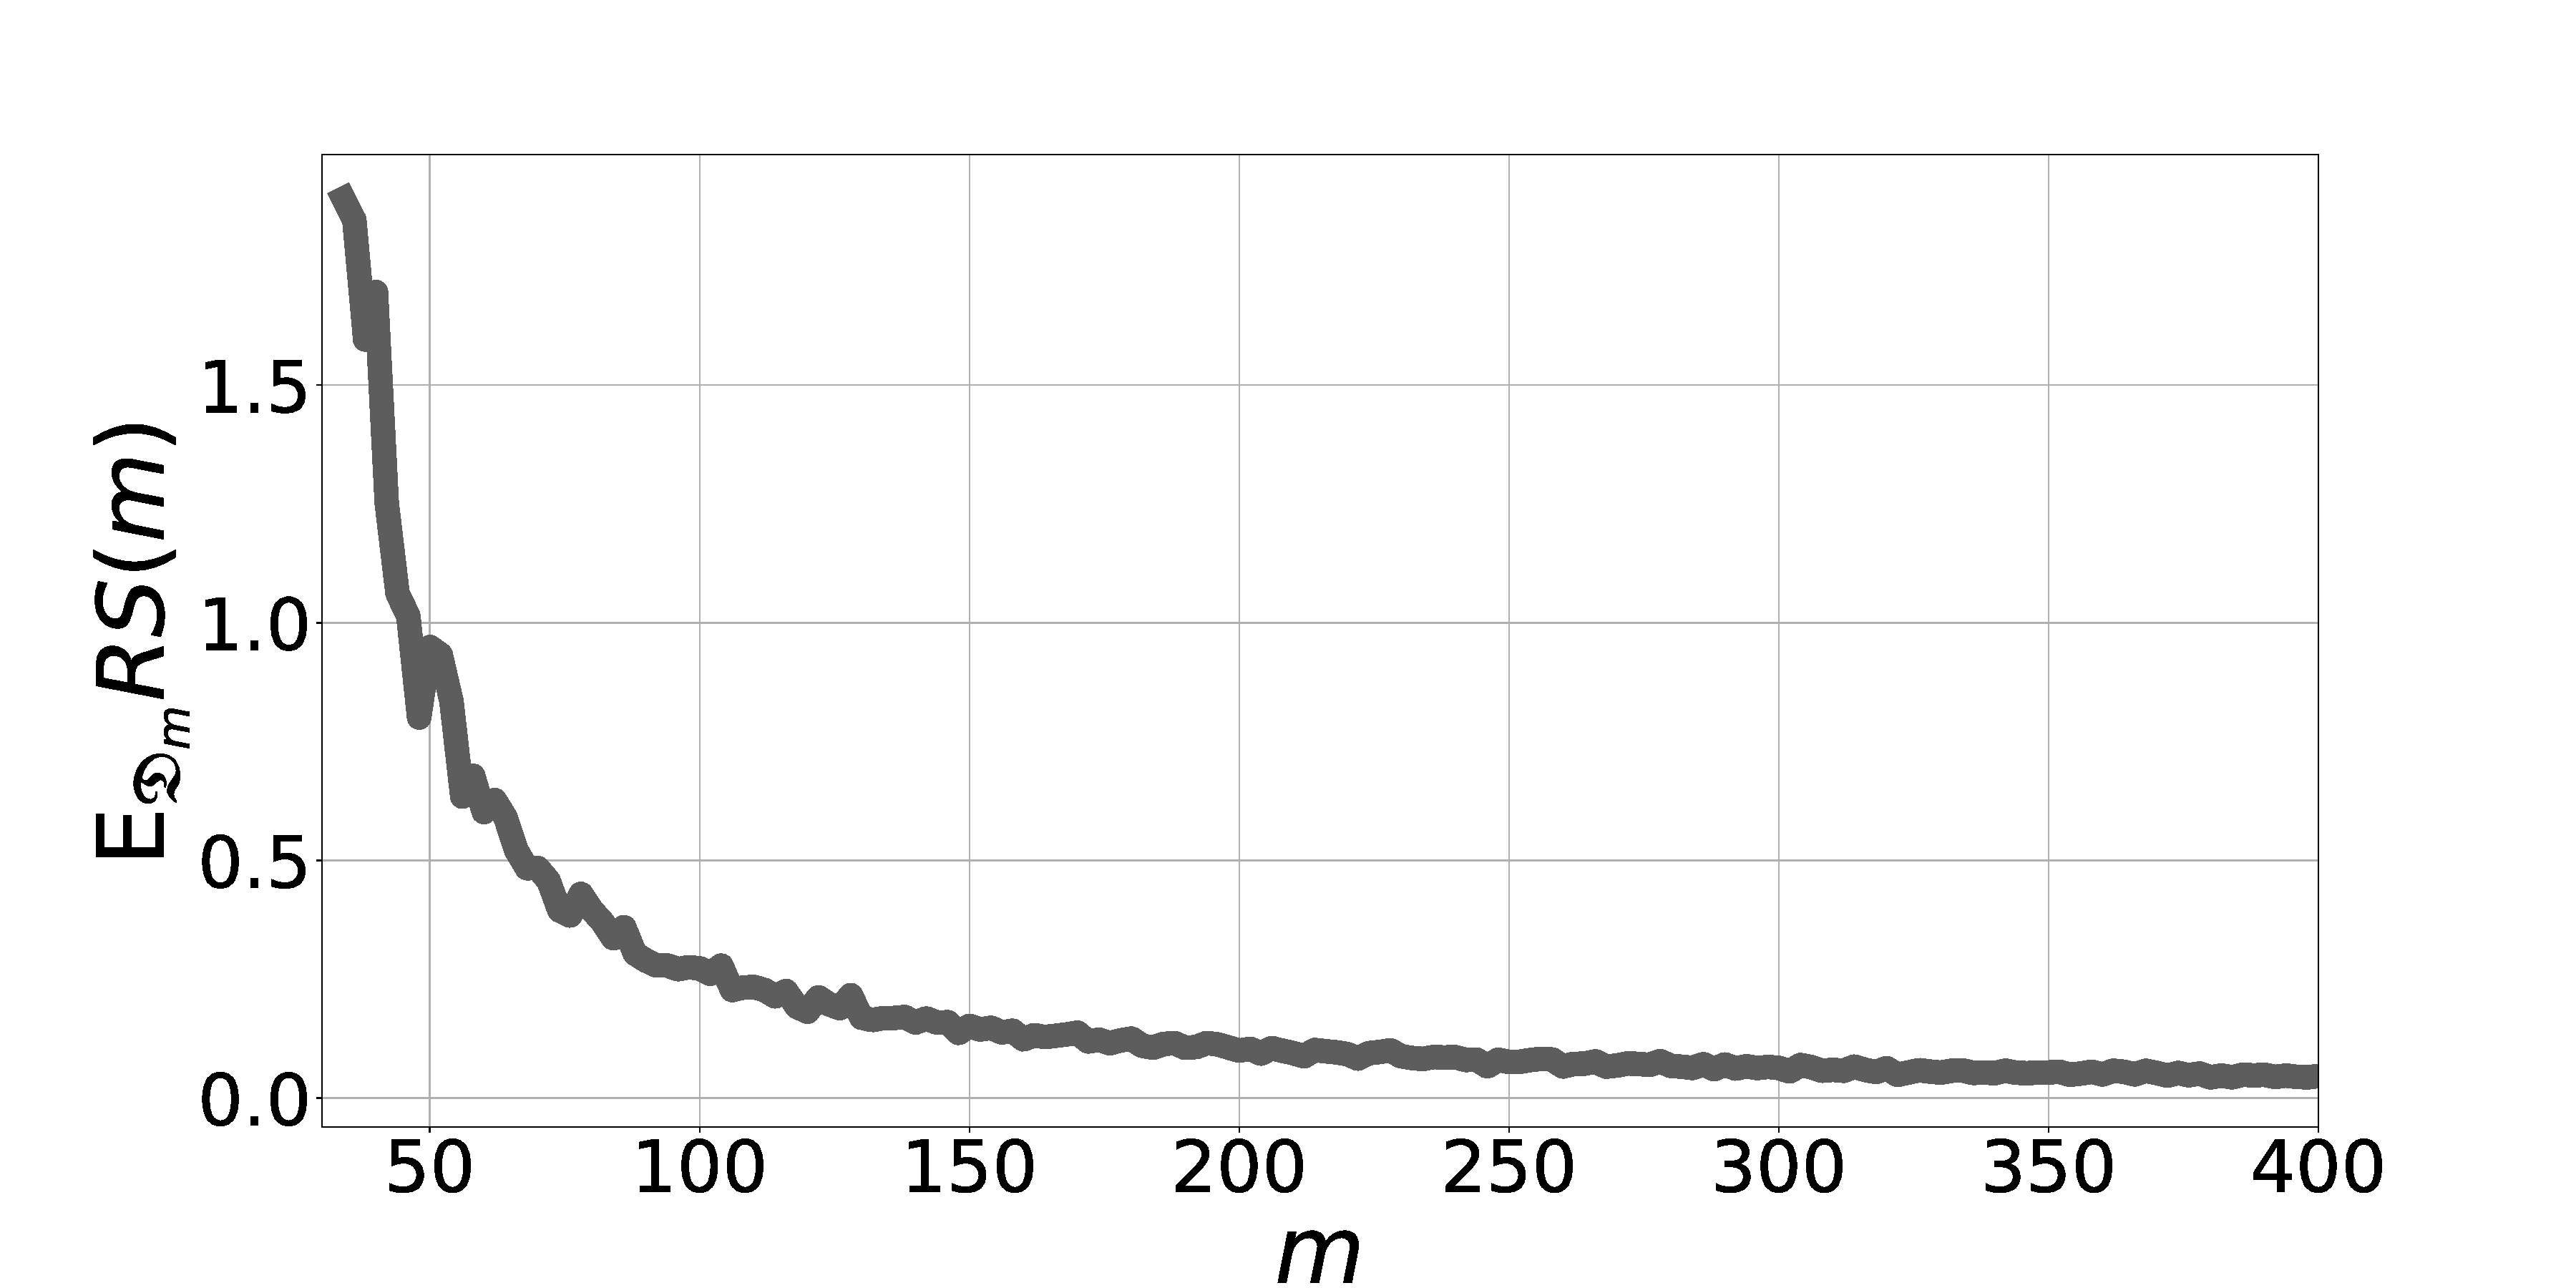
\includegraphics[width=0.49\textwidth]{cross.pdf}}
    \subfloat[APVC ]{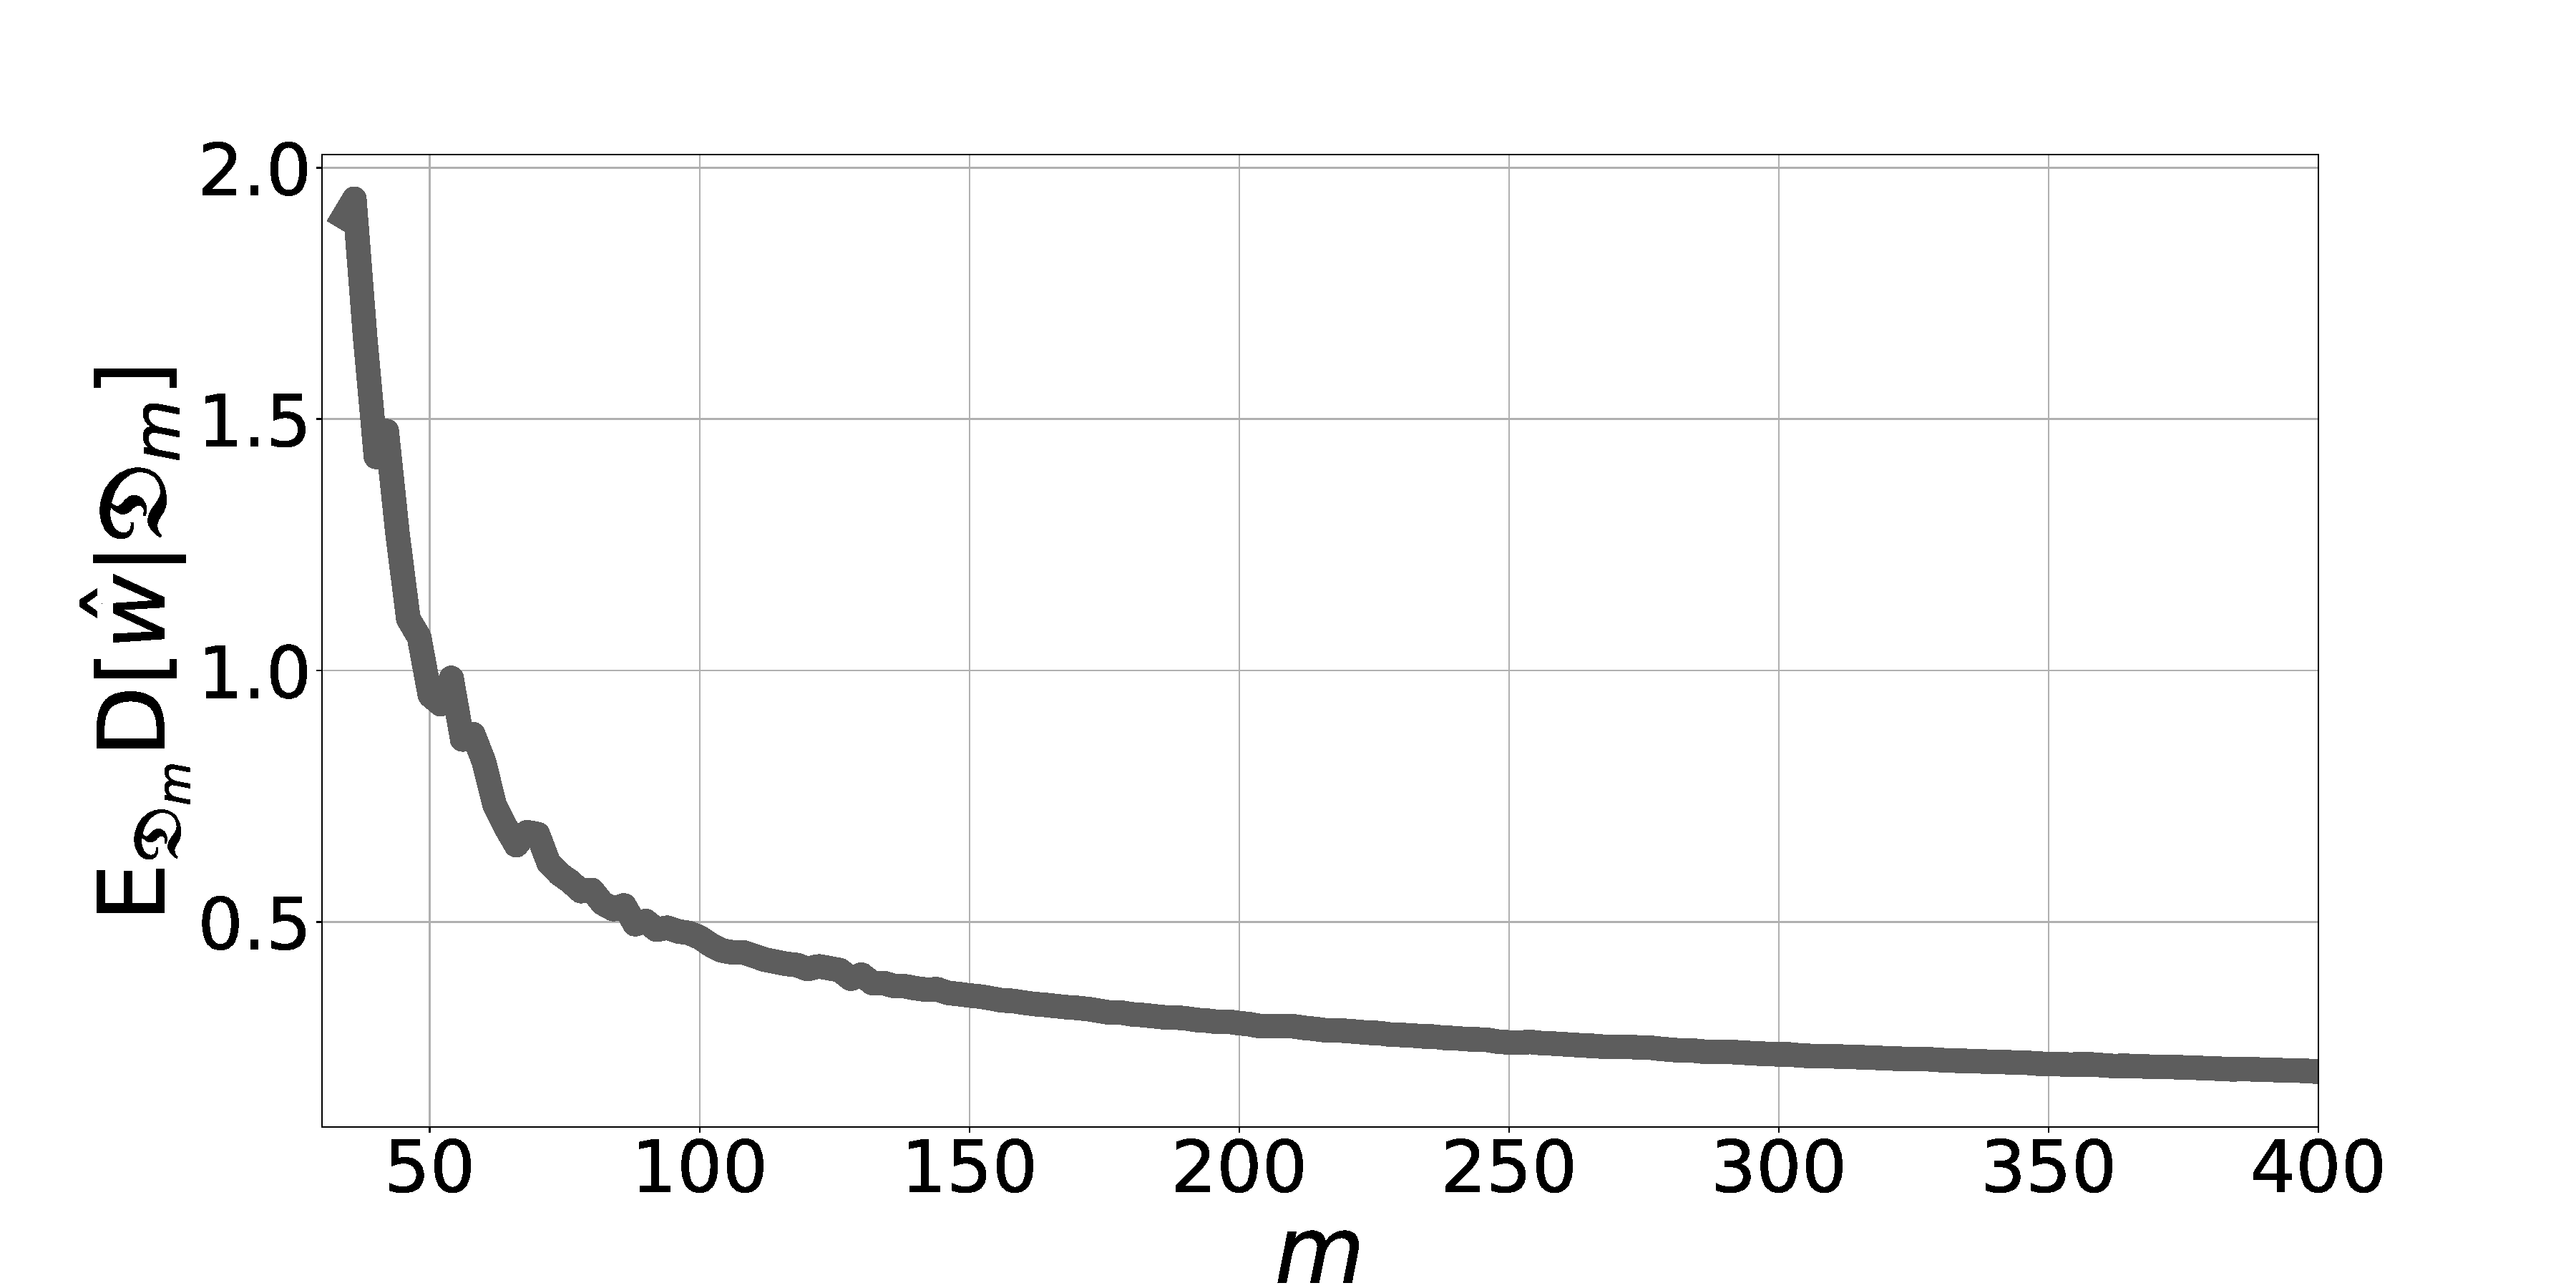
\includegraphics[width=0.49\textwidth]{apvc.pdf}}\\
    \subfloat[ACC ]{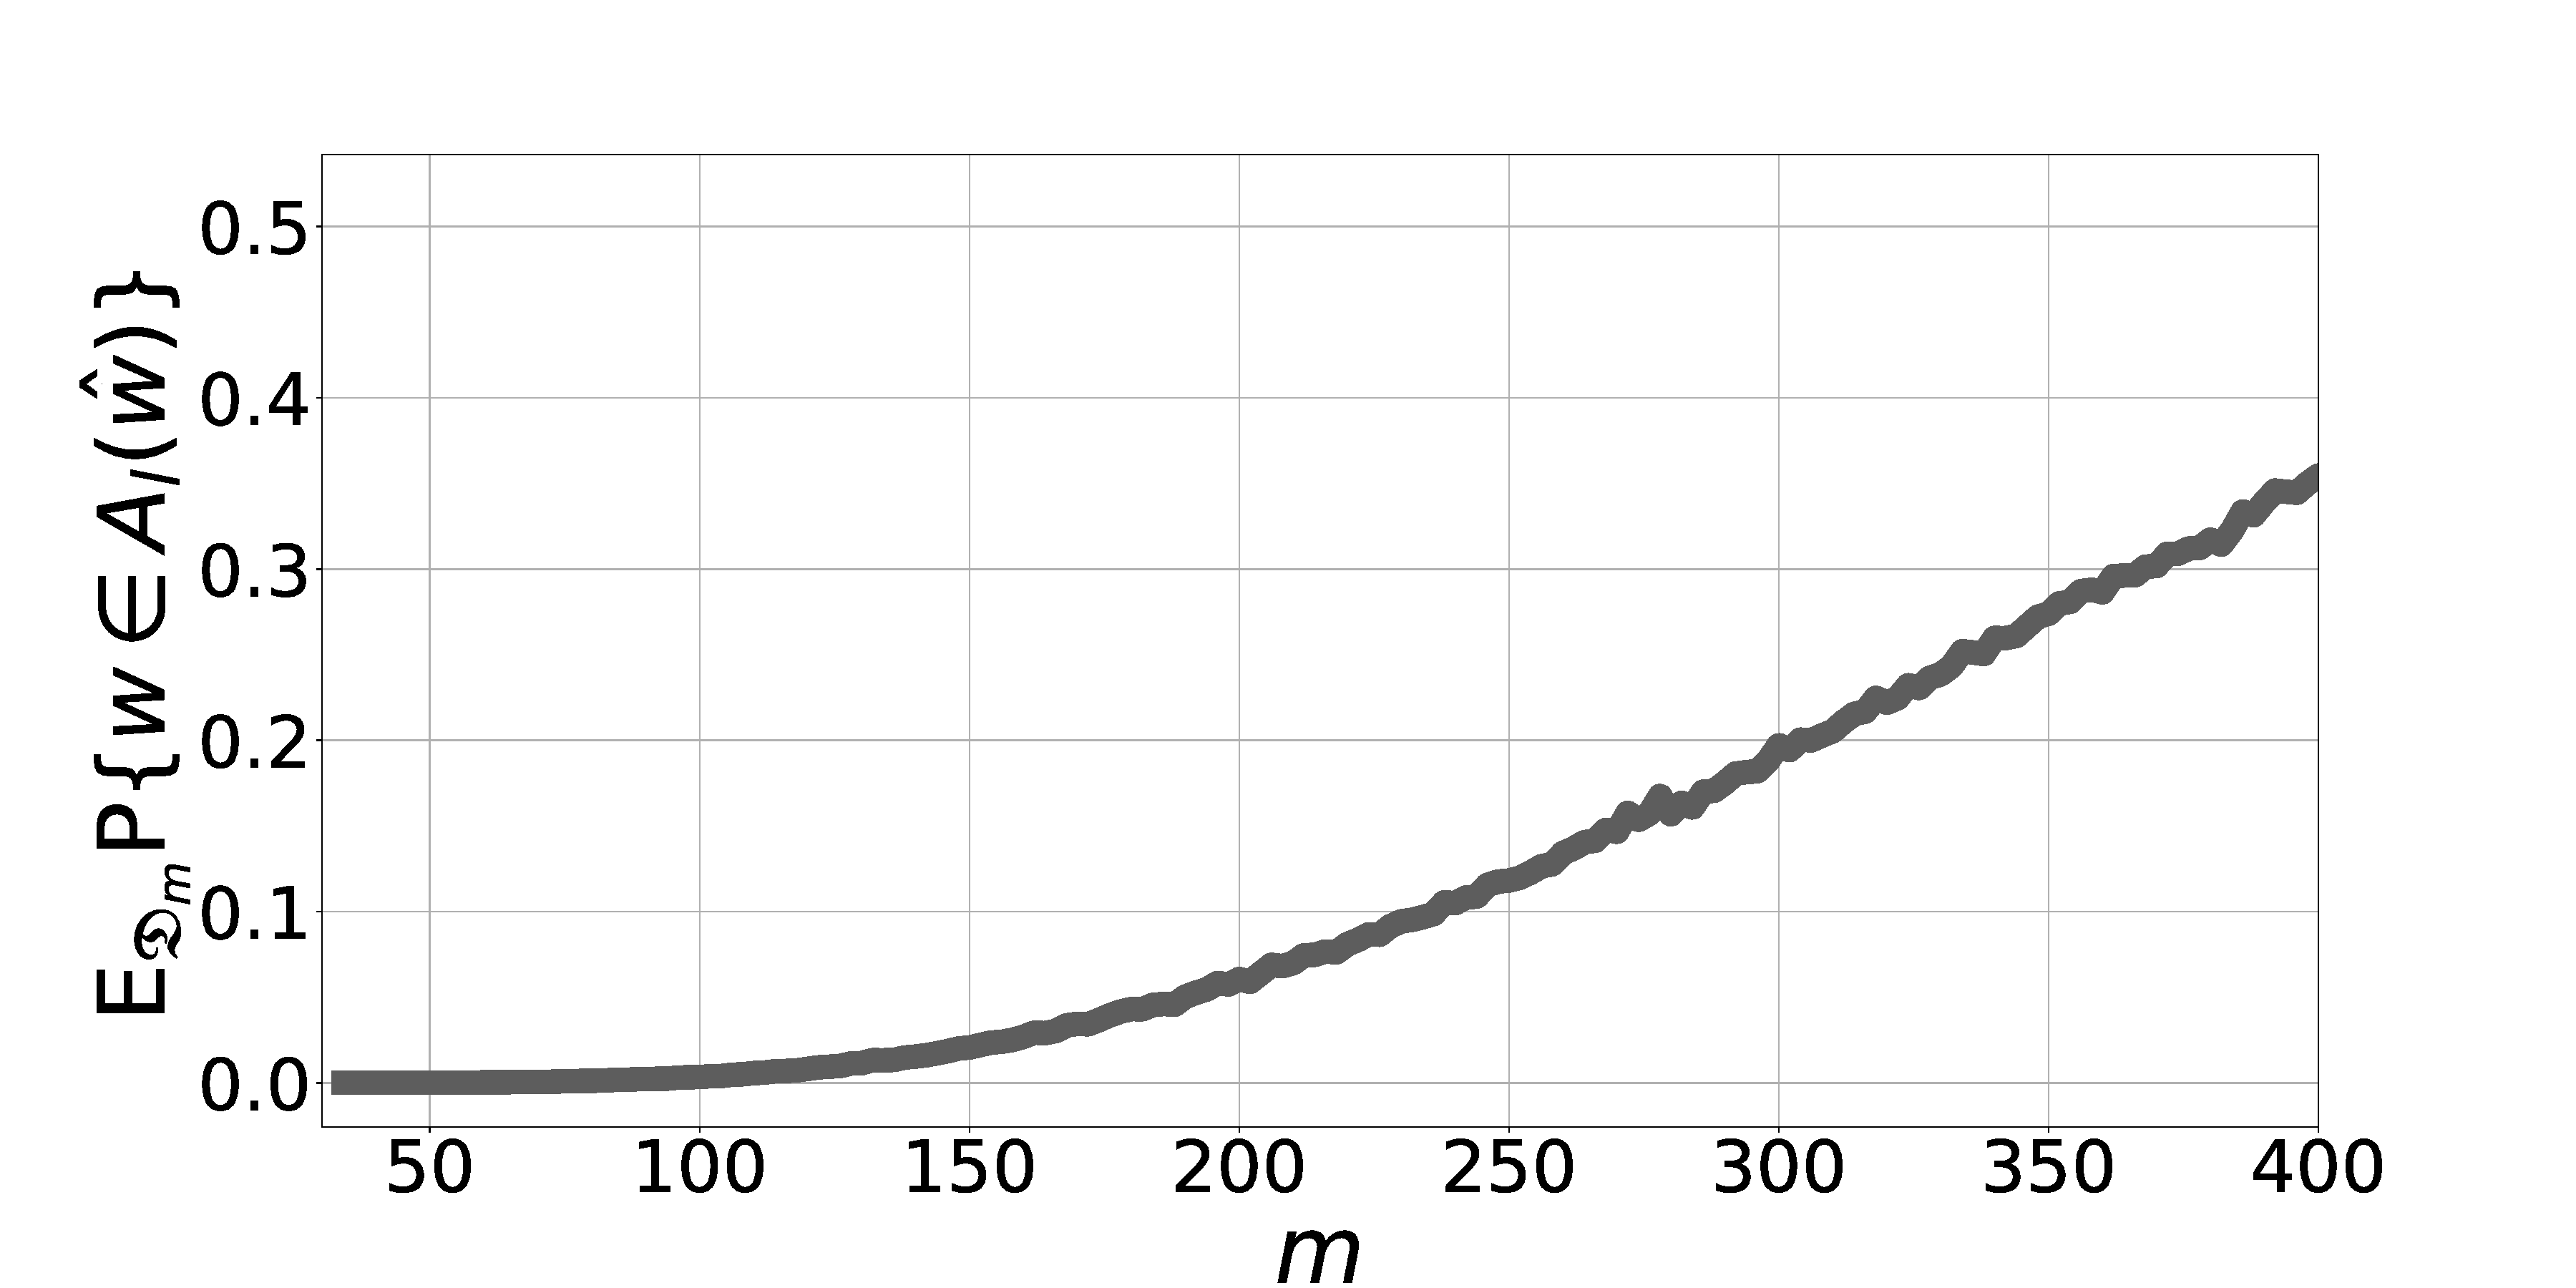
\includegraphics[width=0.49\textwidth]{acc.pdf}}
    \subfloat[ALC ]{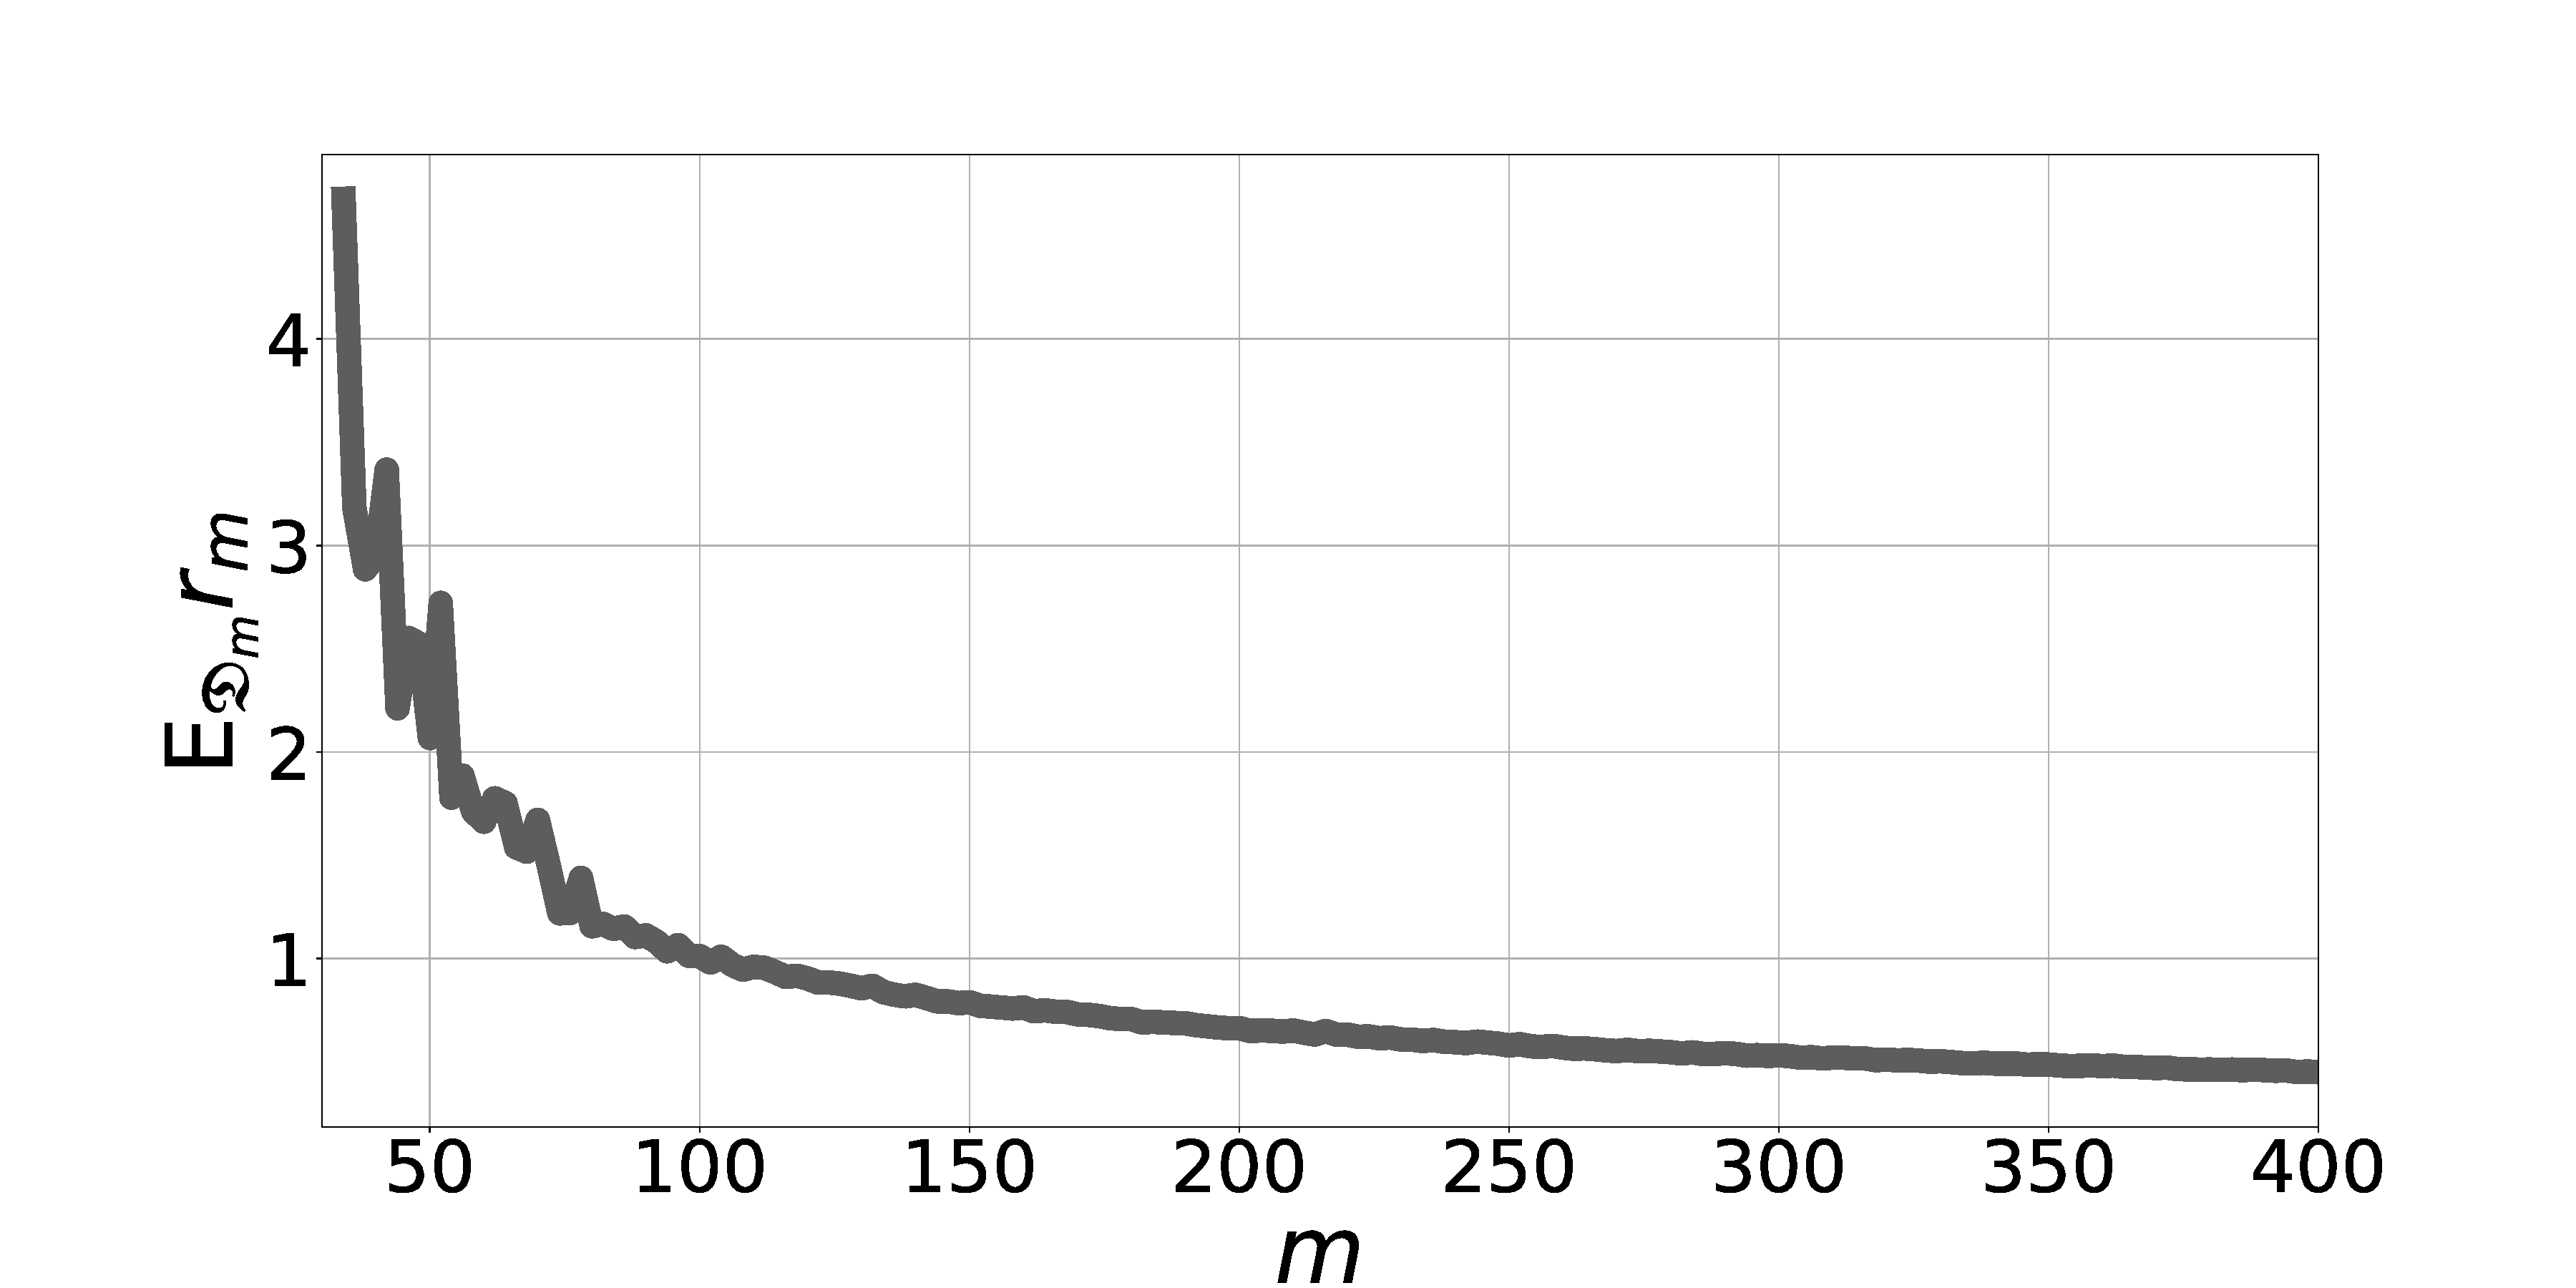
\includegraphics[width=0.49\textwidth]{alc.pdf}}\\
    \subfloat[Bootstrap ]{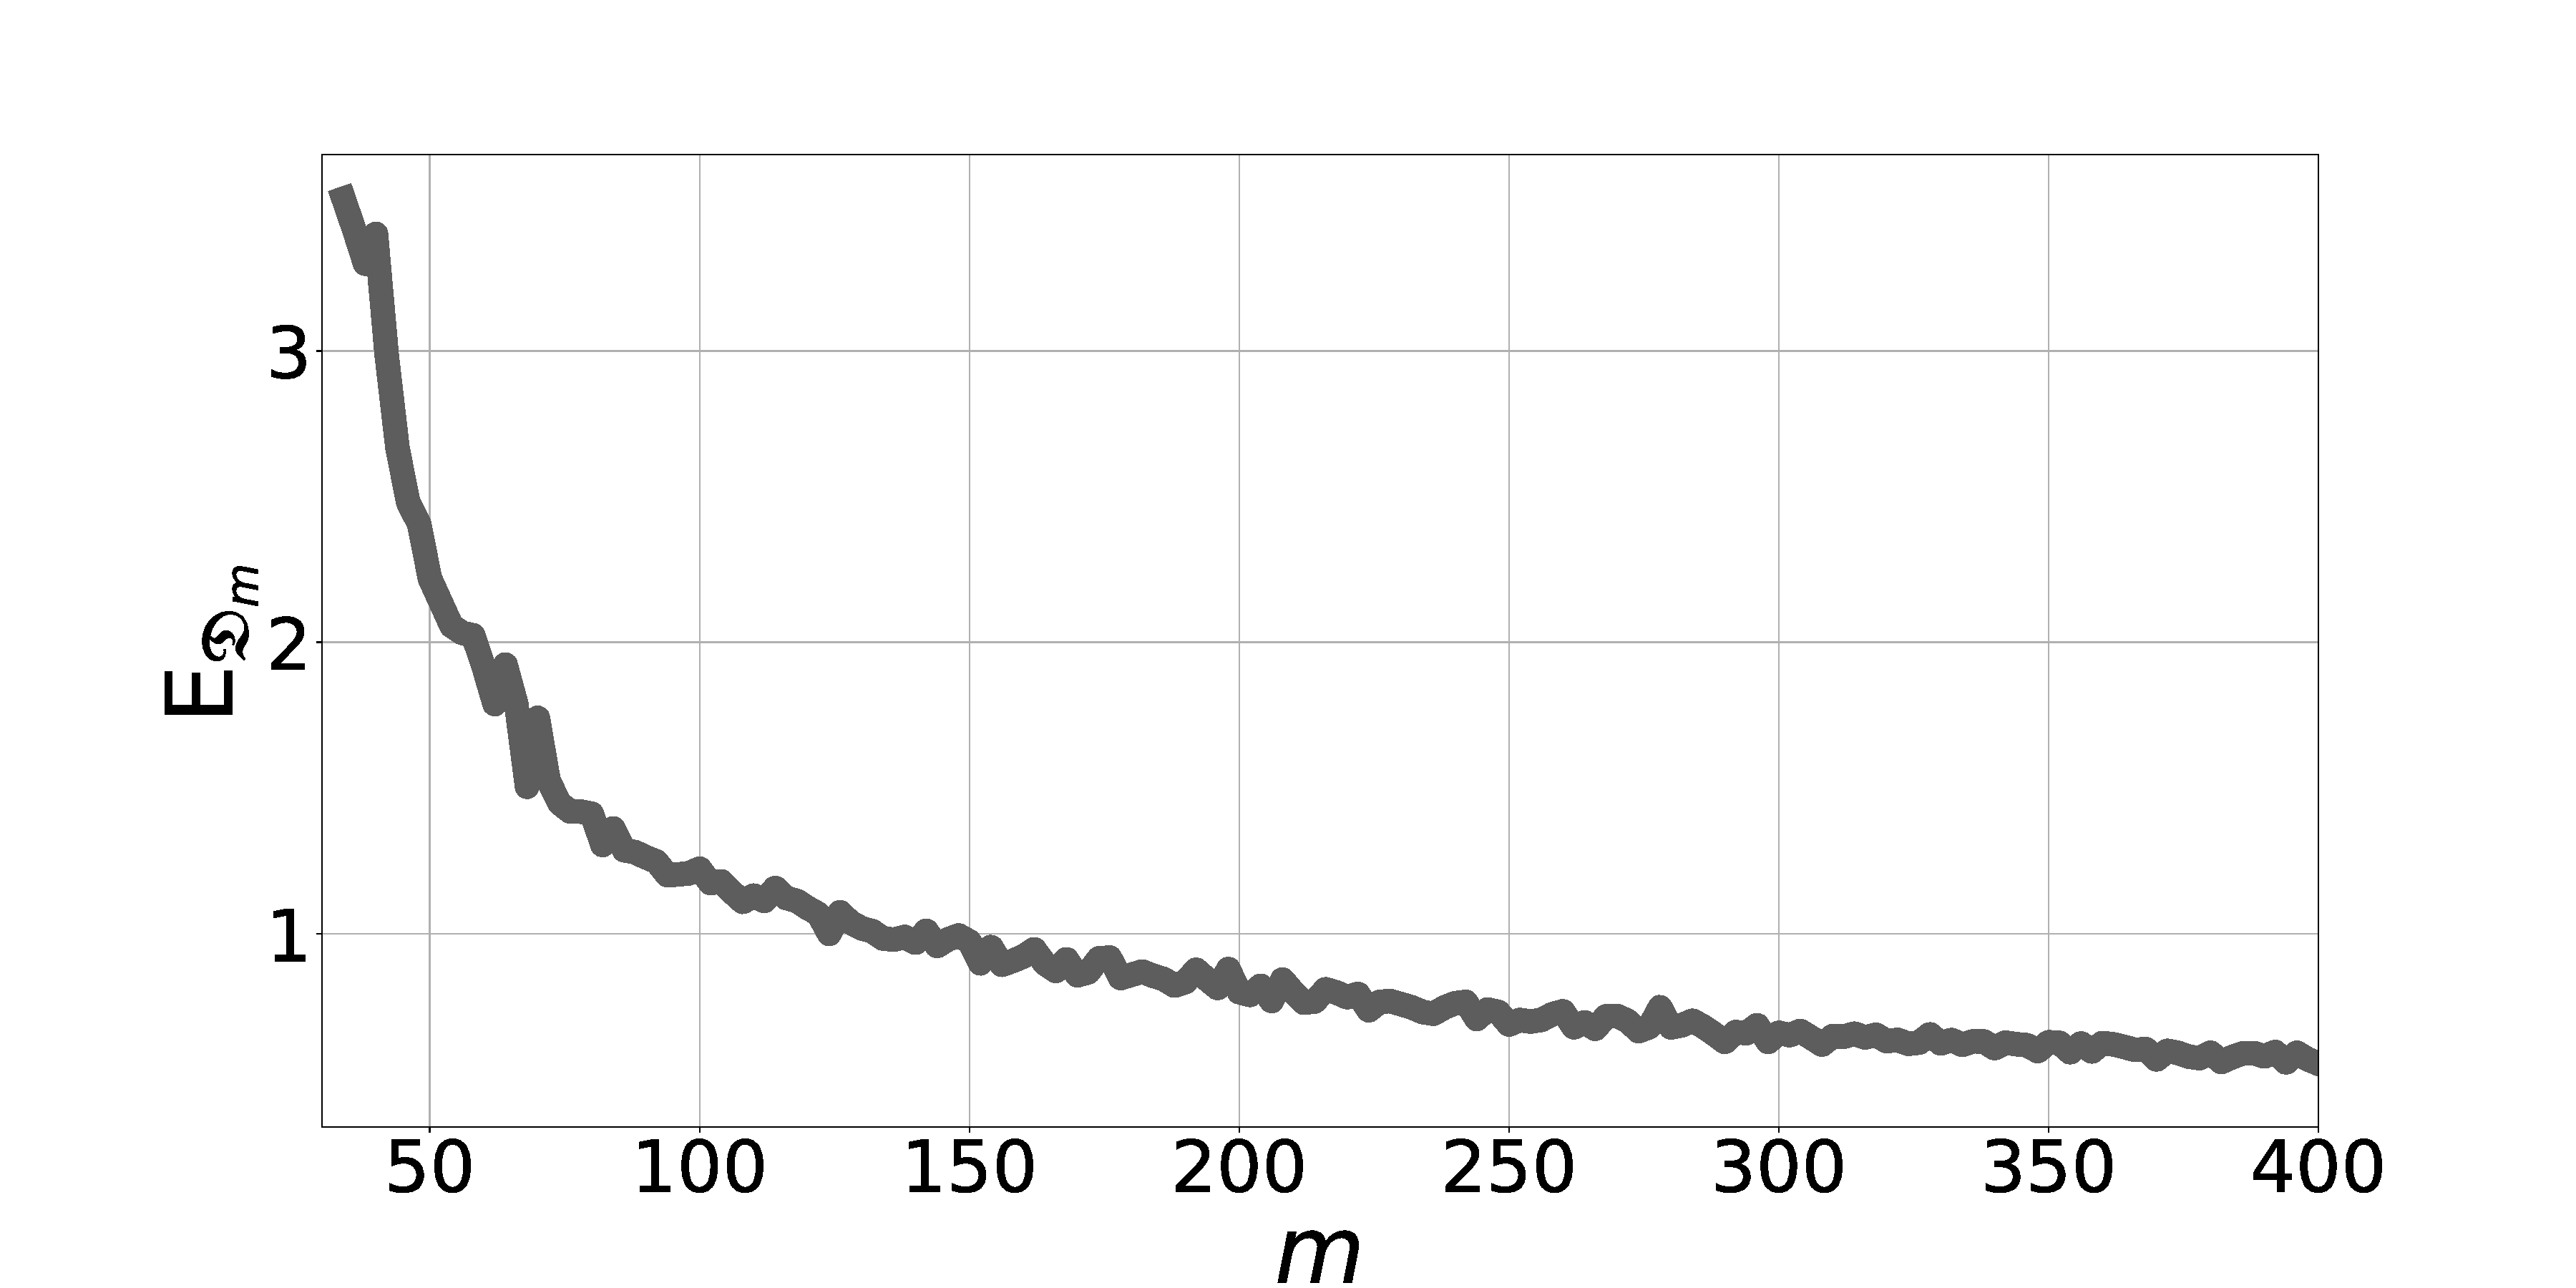
\includegraphics[width=0.49\textwidth]{bootstrap.pdf}}
    \subfloat[KL method ]{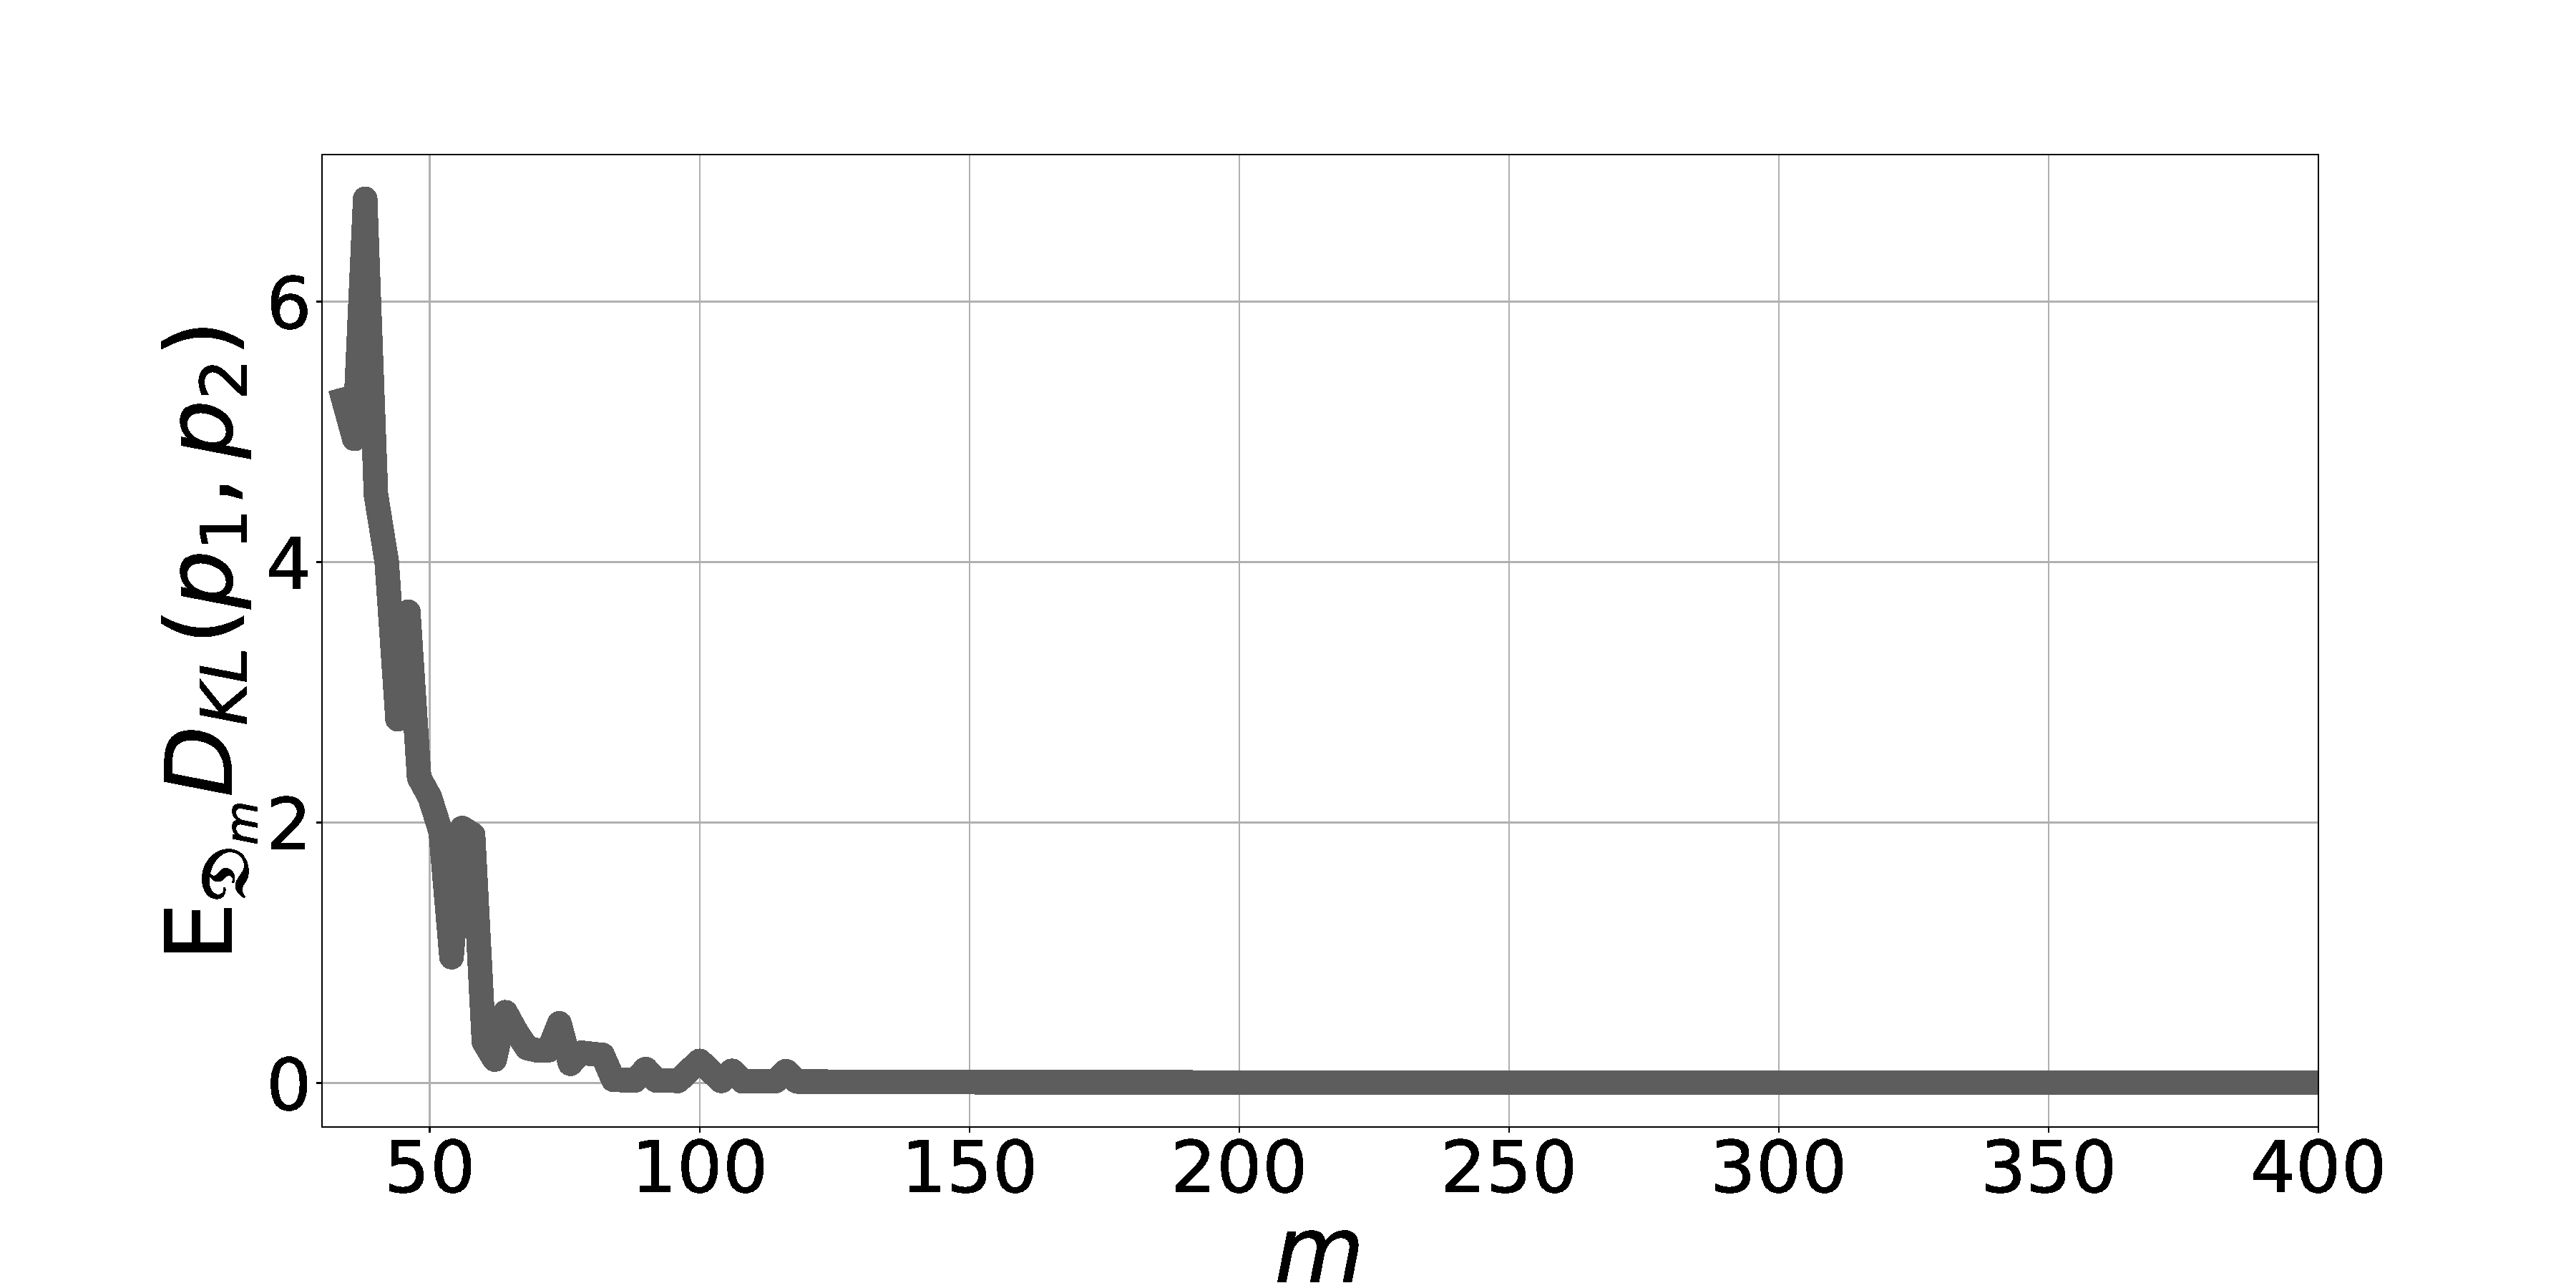
\includegraphics[width=0.49\textwidth]{kl.pdf}}\\
    \subfloat[Utility function ]{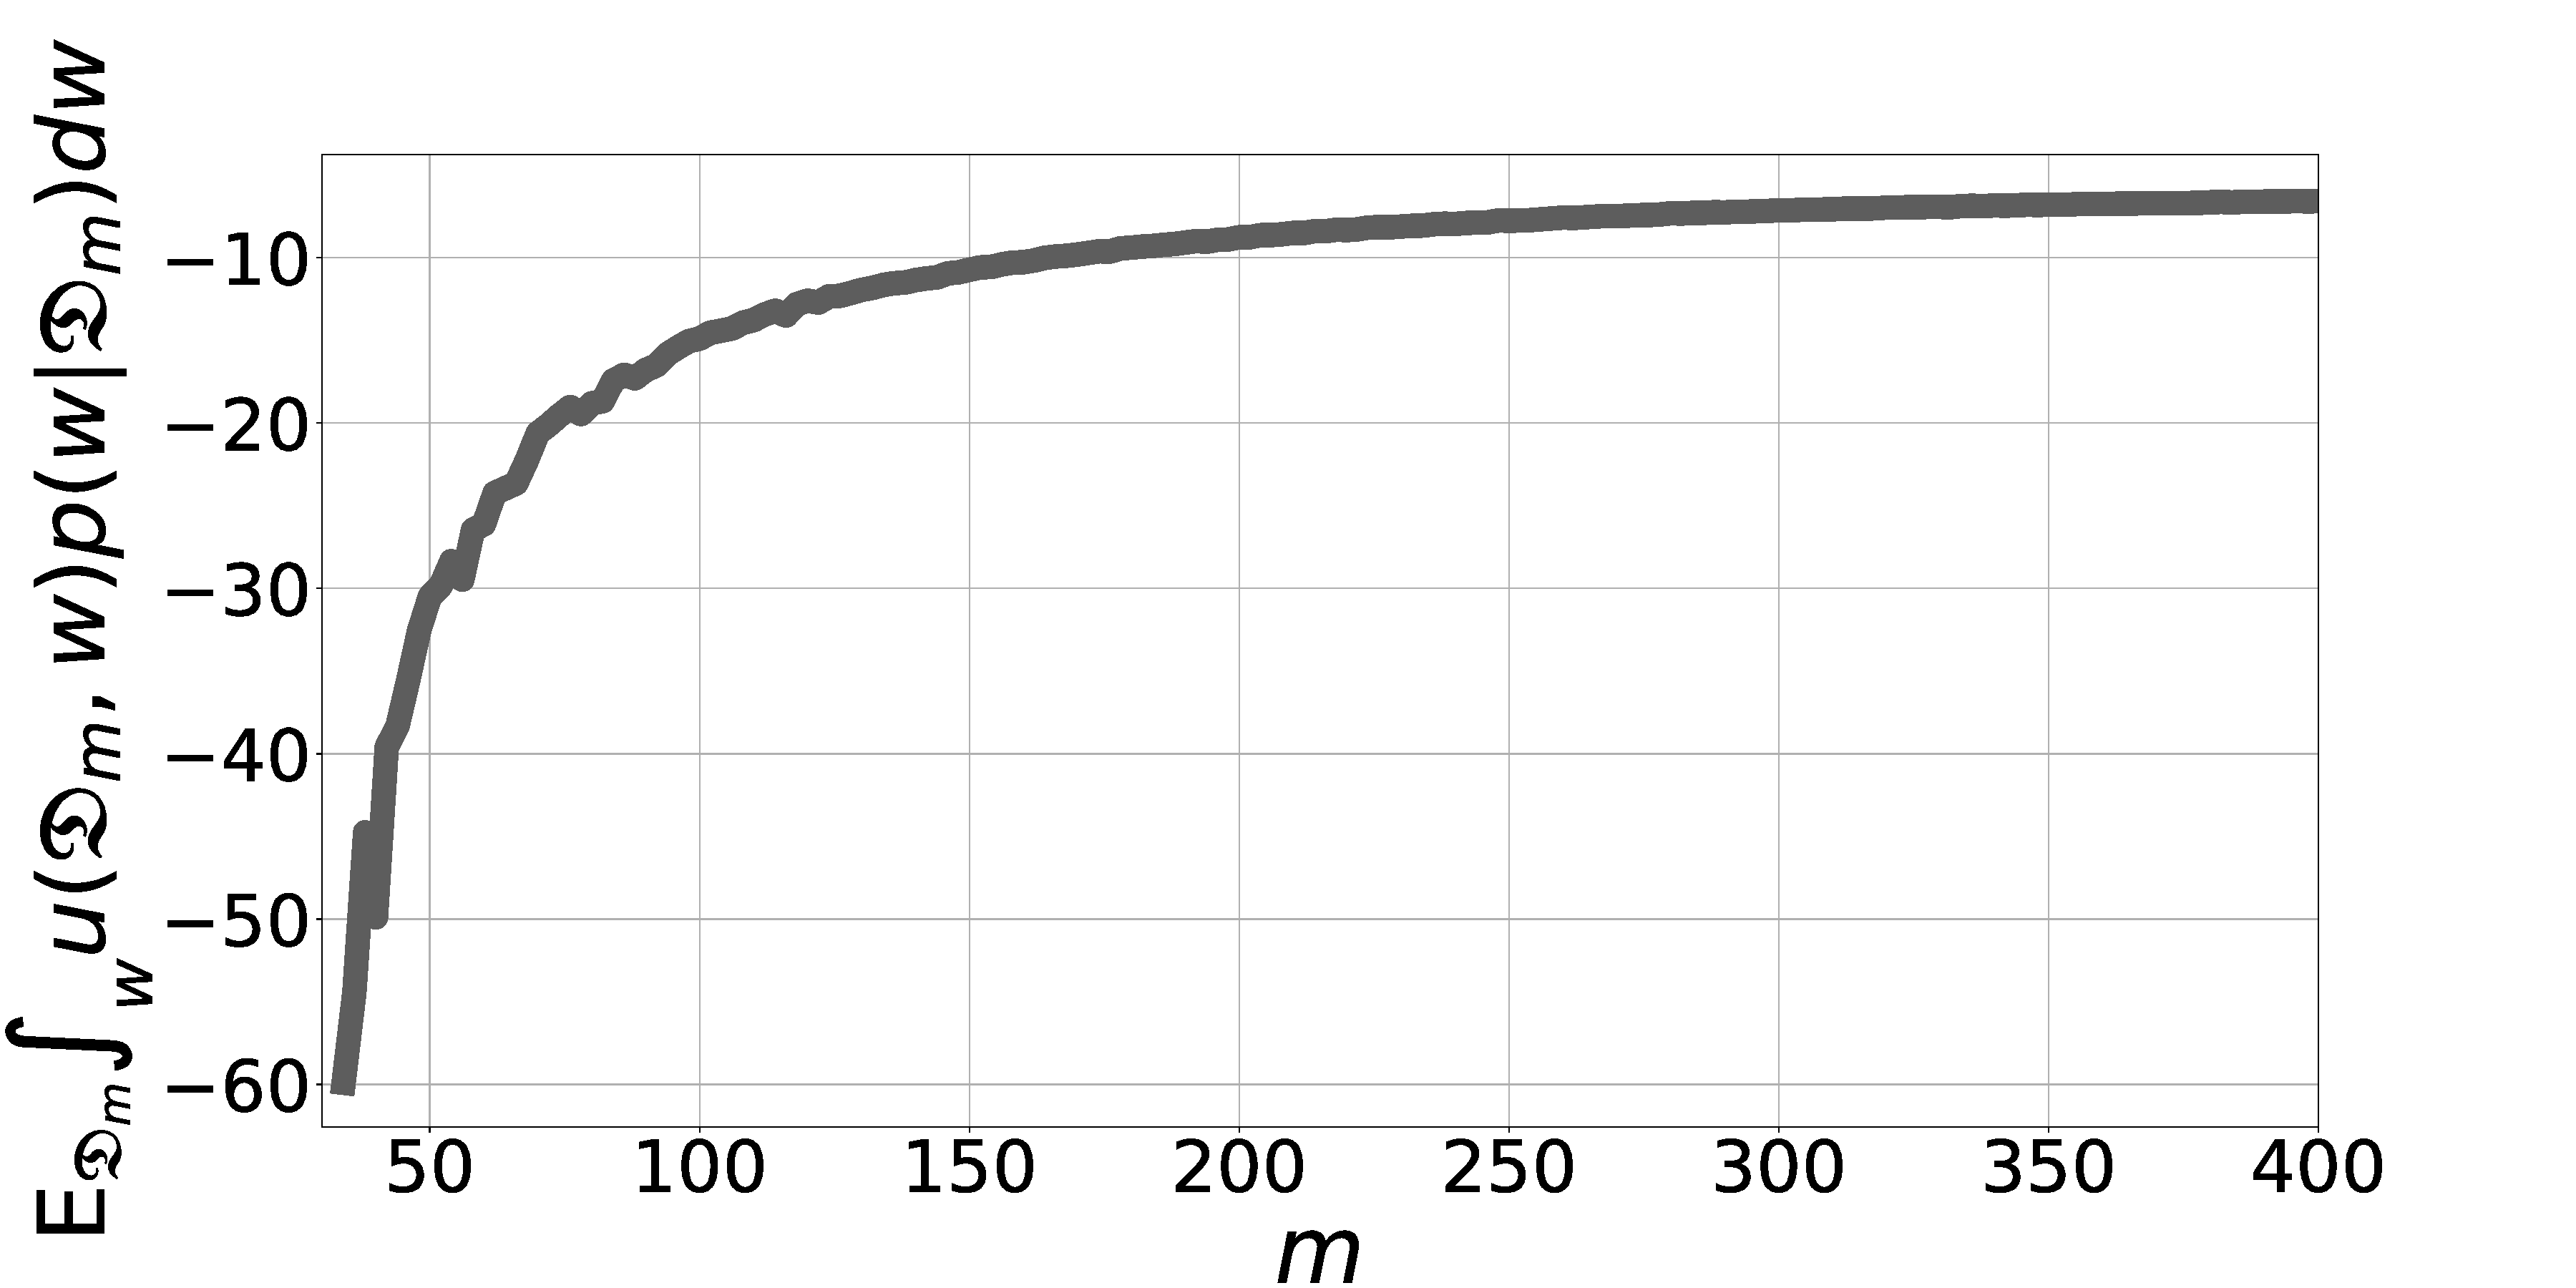
\includegraphics[width=0.49\textwidth]{maxu.pdf}}
    \caption{Methods main scalar functions behaviour dependent on available sample size}
    \label{fig1}
\end{figure}

\begin{figure}[h!t]\center
    {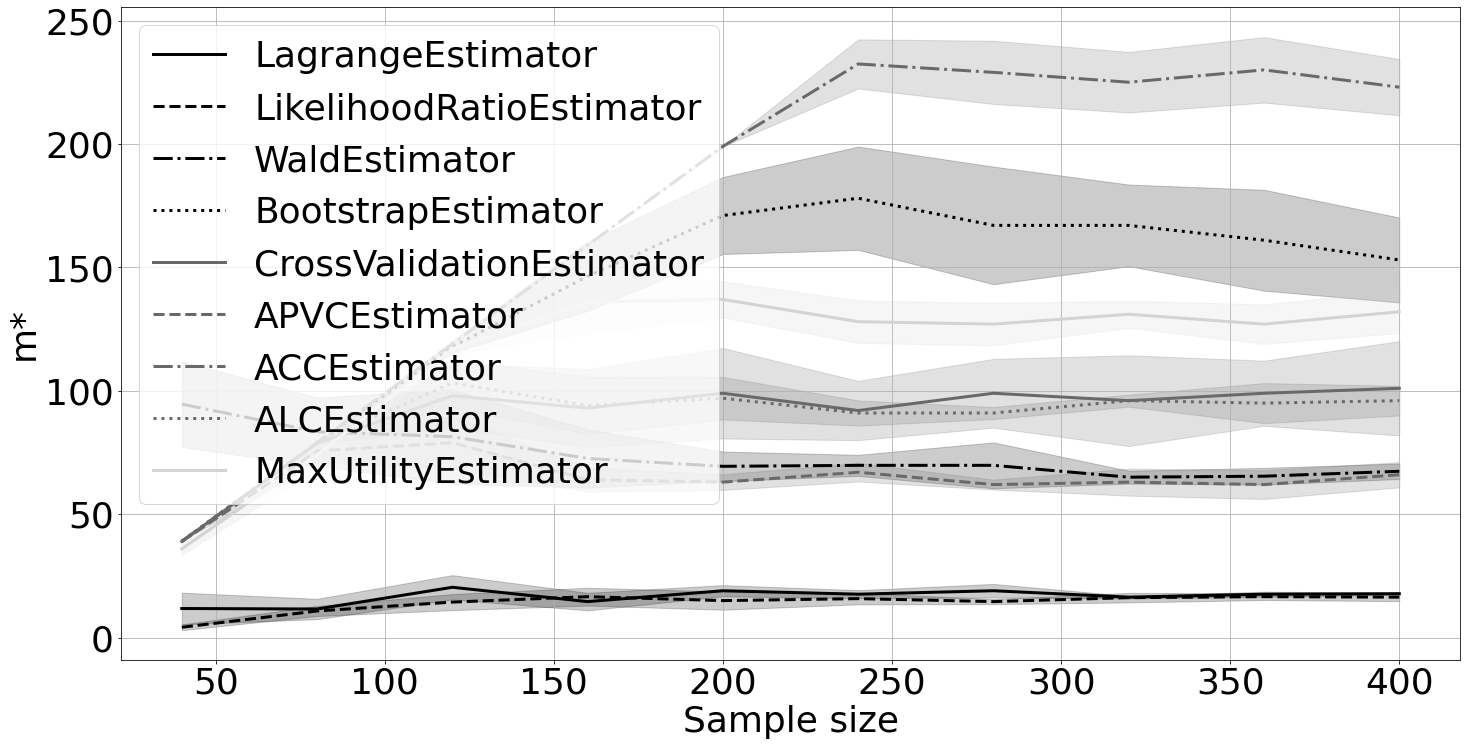
\includegraphics[width=0.85\textwidth]{graphs.png}}
    \caption{Methods behaviour depending on the available sample size}
    \label{fig2}
\end{figure}
    
The Figure~\ref{fig1} shows the dependence of the static values of each method for a given dataset with a fixed sample size $m$. The thresholds for each method are set expertly, which allows us to control different features of the dataset. The figure~\ref{fig1} demonstrates the adequacy of different definitions of sample size sufficiency. All the presented function are monotonous and all of them are asymptotically tend to a constant.
The Figure \ref{fig2} shows methods' results on samples of different size. It shows how methods differ in variance of computed $m^*$ and behaviour in case of small sample set. The methods converge and the result become independent of sample size from some value of $m$. 
    
Small variance interpret as stability of the methods output with little dependency on a particular subsample of some size. Some of the methods can not give estimation of sufficient sample size if they don't have such sample. That means that they are useless in terms of prediction, but can be used for retrospection and analysis of already conducted experiment.

%--- start inclusion
\subsection{Experiment on subsamples}
The dependence between the sample size estimation with the help of a certain method and the volume of data available to this method were considered in this exepriment. The constant achieved by the dependence diagram $m^*$ on $m$ is the forecast of the optimal sample size method. If this constant is less than $m$ where the diagram achieved it, then the method forecasts the optimal sample size before obtaining it. Only Lagrange, Wald methods, and the likelihood ratio method have such property.

\subsection{Experiment on hyperparameter alteration} 
The alteration of the sample size estimation depending on the alteration of certain hyperparameters for Bayesian methods, as well as the methods based on cross-validation and bootstrap is investigated in this experiment. In order to analyse the methods behaviour, see the sample {Boston Housing}, the other samples have the identical tendency.

Bayesian methods, as well as the methods based on cross-validation and bootstrap work on the basis of a certain decision rule for a certain sample function. In the Figure~\ref{fig1}, the dependence of these functions on the subsample size is shown. As shown in the Figure~\ref{fig1}, these functions are monotonically decreasing, or increasing. The function type of behaviour depends on the method. By altering the restrictions set by the application task, the sample size which will comply with these restrictions can be altered.
%--- end inclusion

\section{Software}
Methods of sample size estimation listed above are implemented in a simple Python package. This package can be used both for prediction sufficient sample size in the early stage of the experiment and for retrospective analysis of the sufficiency of the sample set. This package also includes some auxiliary functions for sample size research and visualization of the results such as on the figures above. Source code for sample size estimation service are available at \mbox{\url{https://github.com/andriygav/SampleSizeLib}}. Experiment code and datasets used in the paper are available at \mbox{\url{https://github.com/ttgadaev/SampleSizeEstimation}}.

\section{Conclusion}
In this work, the methods for determining the optimal sample size with the help of frequency and Bayesian methods were investigated. A simulation experiment was performed to investigate the properties of these methods.

As shown in the experiment, the methods used have a series of restrictions. Frequency methods based on the Lagrange tests, likelihood ratio, and Wald tests are asymptotic and cannot be used with little quantity of objects. Bayesian methods, as well as the methods based on cross-validation and bootstrap analyse a certain sample function which requires the greater quantity of objects in order to determine the sample size.

All methods considered require the greater quantity of objects in order to determine the sufficient sample size. It is desired to obtain a criterion which forecasts certain estimation of the sufficient sample size for a smaller quantity of objects, which would make it possible to determine the required quantity of objects for experiment at the early stages of data collection.

\section{Future work}
The main problem is to find a sample size estimation method, that is both interpretable and able to give estimations higher than the available sample set. One of the approaches is to combine Bayesian approach with estimation of statistic on the insufficient sample set. Vector of model parameters are distributed normally. Our future work is to construct a statistic, which estimates mean and covariance matrix of parameters distribution. Such statistic should be estimated on an insufficient sample size in terms of one of the Bayesian definitions of sufficiency. 

\begin{acknowledgments}
This research was supported by Russian Foundation for Basic Research (projects 19-07-01155, 19-07-00875) and National Technological Initiative (project 13/1251/2018).
\end{acknowledgments}

\begin{thebibliography}{}
	\bibitem{demidenko2007}
	E. Demidenko, ``Sample size determination for logistic regression revisited,'' Statist. Med. 26, 3385--3397 (2007).
	
	\bibitem{boston}
	D. Harrison and D. Rubinfeld, ``Hedonic prices and the demand for clean air,'' Economics and Management 5, 81--102 (1978).
	
	\bibitem{joseph1997}
	L. Joseph, R. Berger and P. Be'lisle, ``Bayesian and mixed bayesian likelihood criteria for sample size determination,'' Statistician 16, 769--781 (1995).
	
	\bibitem{joseph1995}
	L. Joseph, D. Wolfson and R. Berger, ``Sample size calculations for binomial proportions via highest posterior density intervals,'' Statistical Medicine 44, 143--154 (1997).
	
	\bibitem{kloek1975}
	T. Kloek, ``Note on a large-sample result in specification analysis,'' Econometrica 43, 933--936  (1975).
	
	\bibitem{lindley1997}
	D. Lindley, ``The choice of sample size,'' Statistician 46, 129--138 (1997).
	
	\bibitem{motrenko2014}
	A. Motrenko, V. Strijov and G. Weber, ``Sample size determination for logistic regression,'' Journal of Computational and Applied Mathematics 255, 743--752 (2014).
	
	\bibitem{servo}
	J. Quinlan, ``Learning with continuous classes,'' in \textit{Proc. 5th Australian Joint Conference on AI} (1992), pp.~343--348.
	
	\bibitem{qumsiyeh2013}
	M. Qumsiyeh, ``Using the bootstrap for estimation the sample size in statistical experiments,'' Journal of modern applied statistical methods 8, 305--321 (2013).
	
	\bibitem{rubin1998}
	D. Rubin and H. Stern, ``Sample size determination using posterior predictive distributions,'' Sankhya: The Indian Journal of Statistics Special Issue on Bayesian Analysis 60, 161--175 (1998).
	
	\bibitem{self1988}
	S. Self and R. Mauritsen, ``Power/sample size calculations for generalized linear models,'' Biometrics 44, 79--86 (1988).
	
	\bibitem{self1992}
	S. Self, R. Mauritsen and J. Ohara, ``Power calculations for likelihood ratio tests in generalized linear models,'' Biometrics 48, 31--39 (1992).
	
	\bibitem{shieh2000}
	G. Shieh, ``On power and sample size calculations for likelihood ratio tests in generalized linear models,'' Biometrics 56, 1192--1196 (2000).
	
	\bibitem{shieh2005}
	G. Shieh, ``On power and sample size calculations for Wald tests in generalized linear models,'' Journal of Statistical Planning and Inference 128, 43--59 (2005).

	\bibitem{wang2002}
	F. Wang and A. Gelfand, ``A Simulation-based Approach to Bayesian Sample Size Determination for Performance under a Given Model and for Separating Models,'' Statistical Science 17, 193--208 (2002).

\end{thebibliography}
\end{document}

